\documentclass[a4paper,11pt]{article}
% ---------------------------------------------------------------
% Preamble: page layout, Persian fonts, headings, boxes, diagrams
% Compile with XeLaTeX (latexmk -xelatex main.tex)
% ---------------------------------------------------------------
\usepackage[a4paper,top=2.6cm,bottom=2.6cm,inner=2.4cm,outer=2.4cm,headheight=24pt]{geometry}
\usepackage{amsmath,amssymb,bm}
\usepackage{graphicx}
\usepackage{xcolor}
\usepackage{booktabs,tabularx,multirow,array}
\usepackage{enumitem}
\usepackage{fancyhdr}
\usepackage{titlesec}
\usepackage[most]{tcolorbox}
\usepackage{tikz}
\usetikzlibrary{arrows.meta,positioning,fit,backgrounds,calc,shapes.geometric}
\usepackage{caption}
\usepackage{float}
\usepackage{pdflscape}
\usepackage[hidelinks]{hyperref}
\graphicspath{{figures/}}
\usepackage{xepersian}   % must be the last package

% ---------- colours ----------
\definecolor{ink}{HTML}{1D1F22}
\definecolor{accent}{HTML}{8C3A22}
\definecolor{accentsoft}{HTML}{F6ECE7}
\definecolor{navy}{HTML}{23395B}
\definecolor{navysoft}{HTML}{E8EDF4}
\definecolor{panel}{HTML}{F4F2EE}
\definecolor{rulegray}{HTML}{BDB7AE}
\definecolor{frozen}{HTML}{E3E8EE}
\definecolor{trainable}{HTML}{F8E6D8}
\definecolor{lossc}{HTML}{E6F0E3}

% ---------- fonts ----------
% XB Niloofar: an installed copy is used first, otherwise fonts/XB-Niloofar.ttf next to main.tex.
% The font has a single weight, so bold and slanted shapes are synthesised.
\IfFontExistsTF{XB Niloofar}{%
  \settextfont[AutoFakeBold=1.6,AutoFakeSlant=0.15]{XB Niloofar}%
}{%
  \settextfont[Path=fonts/,AutoFakeBold=1.6,AutoFakeSlant=0.15]{XB-Niloofar.ttf}%
}
\setlatintextfont[Scale=0.92]{TeX Gyre Termes}
\setlatinsansfont[Scale=0.9]{TeX Gyre Heros}
\setlatinmonofont[Scale=0.85]{Latin Modern Mono}
\linespread{1.45}
\setlength{\parskip}{0.35em}
\setlength{\parindent}{0pt}

% ---------- headings ----------
\titleformat{\section}[block]
  {\color{navy}\LARGE\bfseries}
  {\colorbox{navy}{\color{white}\,\thesection\,}}{0.6em}{}
  [\vspace{2pt}{\color{accent}\titlerule[1.2pt]}]
\titleformat{\subsection}
  {\color{navy}\Large\bfseries}{\color{accent}\thesubsection}{0.6em}{}
\titleformat{\subsubsection}
  {\color{ink}\large\bfseries}{\color{accent}\thesubsubsection}{0.5em}{}
\titlespacing*{\section}{0pt}{2.2em}{1.2em}
\titlespacing*{\subsection}{0pt}{1.6em}{0.6em}
\titlespacing*{\subsubsection}{0pt}{1.2em}{0.4em}
\newcommand{\sectionbreak}{\clearpage}

% ---------- header and footer ----------
\pagestyle{fancy}
\fancyhf{}
\fancyhead[C]{\small\color{navy} \lr{Few-Shot Ordinal-Aware CLIP for Diabetic Retinopathy Grading}}
\fancyfoot[C]{\small\color{navy}\thepage}
\renewcommand{\headrulewidth}{0.4pt}
\renewcommand{\headrule}{{\color{rulegray}\hrule width\headwidth height\headrulewidth}}
\fancypagestyle{plain}{\fancyhf{}\fancyfoot[C]{\small\color{navy}\thepage}\renewcommand{\headrulewidth}{0pt}}

% ---------- captions, numbering ----------
\captionsetup{font=small,labelfont={bf,color=navy},labelsep=colon,skip=6pt}
\captionsetup[table]{position=top}
\numberwithin{equation}{section}
\renewcommand{\arraystretch}{1.3}
\setlist{itemsep=2pt,topsep=4pt}

% ---------- boxes ----------
\newtcolorbox{notebox}[1][]{enhanced,colback=accentsoft,colframe=accent,
  boxrule=0pt,leftrule=0pt,rightrule=3pt,arc=2pt,sharp corners=west,
  fonttitle=\bfseries,coltitle=accent,attach title to upper={\ \ },title={#1},
  left=10pt,right=10pt,top=6pt,bottom=6pt}
\newtcolorbox{keybox}[1][]{enhanced,breakable,colback=navysoft,colframe=navy,
  boxrule=0.6pt,arc=3pt,fonttitle=\bfseries,title={#1},
  left=10pt,right=10pt,top=6pt,bottom=6pt}

% ---------- diagram styles ----------
\tikzset{
  >={Stealth[length=2.4mm]},
  every node/.style={font=\small},
  box/.style={draw=navy!70,rounded corners=3pt,fill=white,align=center,inner sep=4pt,
              text width=#1,minimum height=8mm},
  box/.default=3.4cm,
  frozen/.style={box=#1,fill=frozen},
  frozen/.default=3.4cm,
  train/.style={box=#1,fill=trainable,draw=accent!80},
  train/.default=3.4cm,
  lossn/.style={box=#1,fill=lossc,draw=green!40!black},
  lossn/.default=3.4cm,
  datan/.style={box=#1,fill=panel,draw=rulegray},
  datan/.default=3.4cm,
  decision/.style={diamond,aspect=2.2,draw=accent,fill=accentsoft,align=center,inner sep=1pt,font=\small},
  arr/.style={->,draw=navy!80,thick},
  darr/.style={->,draw=accent!80,thick,dashed},
  group/.style={draw=rulegray,dashed,rounded corners=6pt,inner sep=8pt,fill=panel!50},
  grouplabel/.style={font=\footnotesize\bfseries,text=navy,fill=white,inner sep=2pt},
  elabel/.style={font=\footnotesize,fill=white,inner sep=1pt},
}
\newenvironment{diagram}[1][]{%
  \begin{center}%
  \begin{latin}%
  \begin{tikzpicture}[node distance=7mm and 8mm,#1]%
}{%
  \end{tikzpicture}%
  \end{latin}%
  \end{center}%
}

% legend shown under architecture figures
\newcommand{\archlegend}{%
  \par\smallskip\centering\footnotesize
  \begin{latin}%
  \tikz\node[frozen=1.6cm,minimum height=4mm]{Frozen};\quad
  \tikz\node[train=1.8cm,minimum height=4mm]{Trainable};\quad
  \tikz\node[lossn=1.6cm,minimum height=4mm]{Loss};\quad
  \tikz\node[datan=2.4cm,minimum height=4mm]{Data / Output};\par
  \end{latin}}

% ---------- small helpers ----------
\newcommand{\en}[1]{\lr{#1}}                 % inline Latin text
\newcommand{\code}[1]{\lr{\texttt{#1}}}      % inline code or identifiers
\newcommand{\branch}[1]{\lr{\texttt{#1}}}    % git branch names
\newcommand{\ensent}[1]{\begin{latin}\raggedright\small #1\end{latin}}% Latin sentence in a table cell
\newcolumntype{C}{>{\centering\arraybackslash}X}


\begin{document}

% ================= title page =================
\begin{titlepage}
\begin{tikzpicture}[remember picture,overlay]
  \fill[navy] (current page.north west) rectangle ([yshift=-7.2cm]current page.north east);
  \fill[accent] ([yshift=-7.2cm]current page.north west) rectangle ([yshift=-7.45cm]current page.north east);
  \node[anchor=north,text width=16cm,align=center,text=white,font=\Huge\bfseries] at ([yshift=-2.3cm]current page.north)
    {\lr{Few-Shot Ordinal-Aware CLIP}\\[6pt] \lr{for Diabetic Retinopathy Grading}};
\end{tikzpicture}
\vspace*{7.2cm}

\begin{center}
{\large یک مدل پایه و سه جهت پژوهشی برای یادگیری نمایش ترتیبیِ درجه‌های بیماری\\ در فضای مشترک تصویر و متن\par}
\vspace{1.4cm}

\begin{latin}
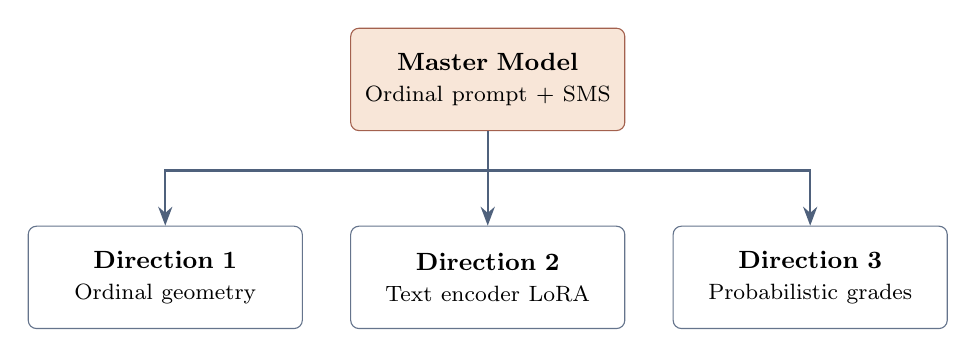
\begin{tikzpicture}[node distance=4mm]
  \node[train=3.2cm,minimum height=13mm] (m) {\textbf{Master Model}\\ \footnotesize Ordinal prompt + SMS};
  \node[box=3.2cm,minimum height=13mm,below=12mm of m] (d2) {\textbf{Direction 2}\\ \footnotesize Text encoder LoRA};
  \node[box=3.2cm,minimum height=13mm,left=6mm of d2] (d1) {\textbf{Direction 1}\\ \footnotesize Ordinal geometry};
  \node[box=3.2cm,minimum height=13mm,right=6mm of d2] (d3) {\textbf{Direction 3}\\ \footnotesize Probabilistic grades};
  \draw[arr] (m.south) -- ++(0,-5mm) -| (d1.north);
  \draw[arr] (m.south) -- (d2.north);
  \draw[arr] (m.south) -- ++(0,-5mm) -| (d3.north);
\end{tikzpicture}
\end{latin}

\vfill
\begin{tabular}{rl}
\textbf{مجموعه‌داده:} & \lr{DeepDRiD} (تصاویر فوندوس معمولی)\\
\textbf{مخزن کد:} & \branch{fewshot-ordinal-clip-dr}\\
\textbf{شاخه‌ها:} & \branch{master}، \branch{direction1-ordinal-geometry}\\
 & \branch{direction2-ordinal-text-lora}، \branch{direction3-probabilistic-ordinal}\\
\textbf{معیار اصلی:} & \lr{Quadratic Weighted Kappa (QWK)} و افت خطا با فاصله از قطر\\
\end{tabular}
\vspace{1cm}
\end{center}
\end{titlepage}

\pagenumbering{alph}
\tableofcontents
\clearpage
\listoffigures
\listoftables
\clearpage
\pagenumbering{arabic}

\section*{مقدمه و نقشهٔ سند}
\addcontentsline{toc}{section}{مقدمه و نقشهٔ سند}
\markboth{مقدمه}{مقدمه}

رتینوپاتی دیابتی (\lr{Diabetic Retinopathy, DR}) بر اساس مقیاس بین‌المللی \lr{ICDR} در پنج درجه سنجیده می‌شود: بدون رتینوپاتی، خفیف، متوسط، شدید غیرتکثیری و تکثیری. این درجه‌ها ترتیب دارند. اشتباه گرفتن درجهٔ ۱ با درجهٔ ۲ از نظر بالینی بسیار کم‌هزینه‌تر از اشتباه گرفتن درجهٔ ۰ با درجهٔ ۴ است؛ با این حال بیشتر \lr{classifier}ها درجه‌ها را برچسب‌هایی مستقل می‌بینند و این ساختار را نادیده می‌گیرند. مشکل دوم کمبود داده است: برچسب‌زدن تصویر فوندوس به چشم‌پزشک نیاز دارد و در عمل گاهی فقط چند تصویر برای هر درجه در دسترس است.

مدل‌های بینایی و زبان مانند \lr{CLIP} \cite{clip} برای \lr{regime} \lr{few-shot} مناسب‌اند، چون دانش زبانی‌شان دربارهٔ مفاهیم را می‌توان با چند نمونه به یک مسئلهٔ تازه منتقل کرد. پرسش این پژوهش این است که ترتیب درجه‌ها را کجا و چگونه باید در این فضای مشترک وارد کرد تا مدل با تعداد بسیار کمی تصویر، درجه‌ها را نه‌تنها درست، بلکه با خطاهای «نزدیک» پیش‌بینی کند. \lr{metric} اصلی موفقیت در همهٔ بخش‌ها \lr{Quadratic Weighted Kappa} (\lr{QWK}) است و در کنار آن بررسی می‌شود که در \lr{confusion matrix}، خطاها با دور شدن از قطر اصلی کاهش یابند.

سند در چهار بخش اصلی تنظیم شده است. هر بخش یک مدل کامل است و برای خواندن مستقل نوشته شده؛ اجزای مشترک در بخش~\ref{sec:master} با جزئیات کامل آمده و در بخش‌های بعد، همراه با اعداد کلیدی، خلاصه شده است.

\begin{keybox}[پرسش‌های پژوهش]
\begin{enumerate}[label=\arabic*.]
\item آیا ترتیب درجه‌ها، اگر در \lr{prompt}، \lr{loss} و \lr{similarity statistic} با هم وارد شود، در \lr{regime} \lr{few-shot} \lr{QWK} را بهبود می‌دهد؟ (بخش~\ref{sec:master})
\item آیا اعمال ترتیب مستقیماً روی هندسهٔ \lr{prototype}ها درجه‌ها، به‌جای ورودی \lr{text encoder}، مؤثرتر است؟ (بخش~\ref{sec:d1})
\item آیا تطبیق خود \lr{text encoder} با توصیف‌های بالینی، همراه با \lr{constraint} ترتیبی روی خروجی آن، نمایش بهتری می‌سازد؟ (بخش~\ref{sec:d2})
\item آیا نمایش احتمالاتی درجه‌ها، با \lr{concentration} \lr{trainable} برای هر درجه، هم دقت ترتیبی و هم \lr{calibration} را بهبود می‌دهد؟ (بخش~\ref{sec:d3})
\end{enumerate}
\end{keybox}

\begin{figure}[H]
\begin{diagram}
  \node[datan=6cm] (p) {\textbf{Problem:} Ordinal DR Grading\\ with few images per grade};
  \node[train=7.2cm,below=of p] (m) {\textbf{Sec.~1 · Master}\\ Ordinal prompt + image LoRA + rank-aware loss + SMS};
  \node[box=4.3cm,below=12mm of m] (d2) {\textbf{Sec.~3 · Dir.~2}\\ Clinical descs.\ + text LoRA + ordinal constraint on text output};
  \node[box=4.3cm,left=5mm of d2] (d1) {\textbf{Sec.~2 · Dir.~1}\\ Grade vectors directly in shared space + geometric ordinal constraints};
  \node[box=4.3cm,right=5mm of d2] (d3) {\textbf{Sec.~4 · Dir.~3}\\ Per-grade vMF distribution + learnable concentration};
  \node[lossn=9cm,below=12mm of d2] (e) {\textbf{Shared evaluation:} QWK · MAE · ODC · ECE · NLL};
  \draw[arr] (p) -- (m);
  \foreach \d in {d1,d2,d3} {\draw[arr] (m.south) -- ++(0,-5mm) -| (\d.north); \draw[arr] (\d.south) -- (\d.south |- e.north);}
\end{diagram}
\caption{چهار مدل پژوهش و ارتباط آن‌ها. هر سه جهت بر \lr{image branch}، داده، \lr{protocol} و \lr{metric}های مدل پایه بنا شده‌اند و فقط در نحوهٔ ساختن نمایش متنیِ درجه‌ها تفاوت دارند.}
\label{fig:overview}
\end{figure}

\begin{table}[H]
\caption{چهار مدل در یک نگاه}
\label{tab:glance}
\centering\small
\begin{tabularx}{\textwidth}{@{}l X X r@{}}
\toprule
\textbf{مدل} & \textbf{نمایش متنی درجه‌ها از کجا می‌آید} & \textbf{ترتیب کجا اعمال می‌شود} & \textbf{\lr{parameter} \lr{trainable}}\\
\midrule
مدل پایه & \lr{prompt} با \lr{context token}ها و رتبهٔ \lr{learnable}، از \lr{text encoder} \lr{frozen} & \lr{interpolation} \lr{rank token}ها، \lr{ranking-aware loss}، \lr{SMS} & \LRE{۱٬۱۹۸٬۰۰۰}\\
جهت ۱ & پنج بردار آزاد در فضای مشترک، آغازشده از جمله‌های بالینی & \lr{constraint}های \lr{ladder}، \lr{path} و \lr{anchor} روی خود بردارها & \LRE{۱٬۱۹۳٬۳۹۲}\\
جهت ۲ & میانگین ۵ توصیف بالینی برای هر درجه، از \lr{text encoder} تطبیق‌یافته با \lr{LoRA} & \lr{ladder} روی \lr{prototype}ها، \lr{description ordering}، \lr{anchor} & \LRE{۱٬۲۶۲٬۰۰۰}\\
جهت ۳ & \lr{von Mises--Fisher distribution} برای هر درجه: \lr{mean direction} و \lr{concentration} & \lr{ladder} و \lr{anchor} روی میانگین‌ها، \lr{overlap} توزیع‌ها & \LRE{۱٬۱۹۳٬۳۹۷}\\
\bottomrule
\end{tabularx}
\end{table}

\section{مدل پایه (شاخهٔ \lr{master})}
\label{sec:master}

شکل~\ref{fig:wf-master} کل گردش کار مدل پایه را در یک نگاه نشان می‌دهد: \lr{block}های مدل (الف) و \lr{loss function}، \lr{calibration} و ارزیابی (ب). تقسیم داده در بخش~\ref{sec:data} و \lr{protocol} آزمایش‌ها در شکل~\ref{fig:proto-master} جداگانه آمده‌اند و زیربخش‌های این فصل هر \lr{block} را شرح می‌دهند.

\begin{landscape}
\begin{figure}[p]
\centering
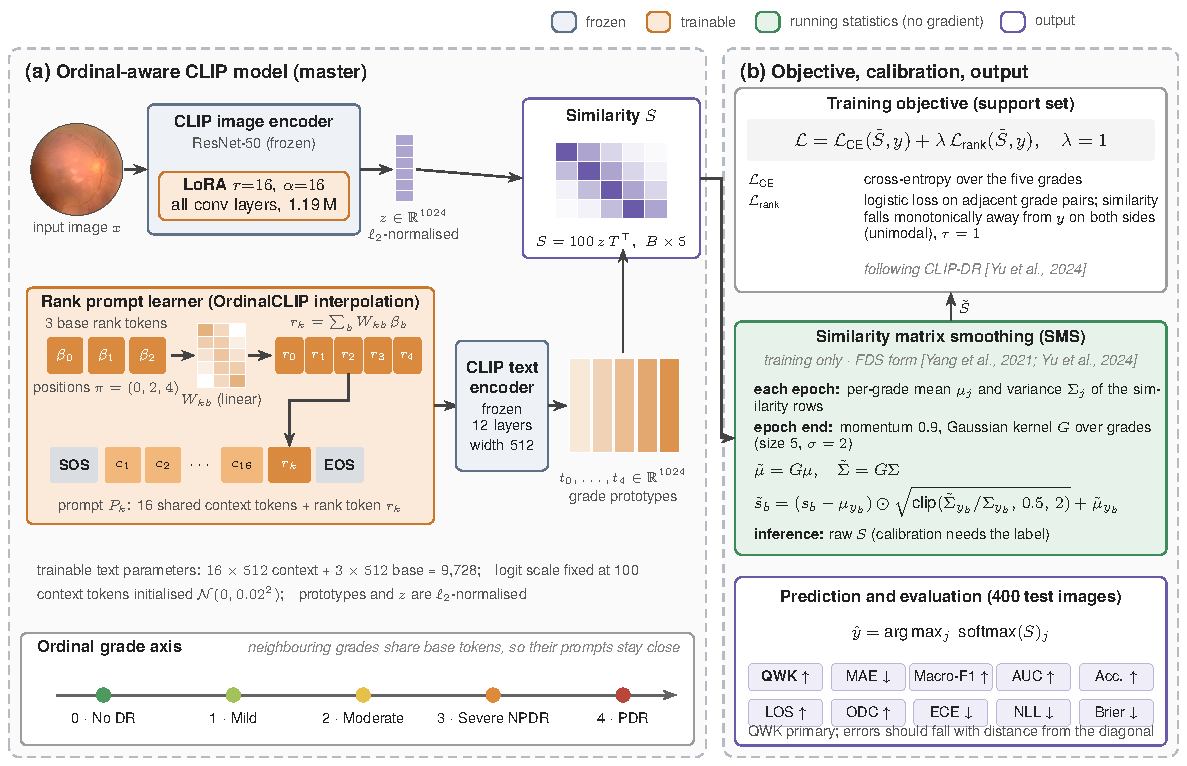
\includegraphics[width=\linewidth]{workflow_master}
\caption{گردش کار کامل مدل پایه: (الف) \lr{image branch} با \lr{LoRA} و \lr{prompt learner} رتبه‌ای \lr{OrdinalCLIP}، (ب) \lr{cross-entropy} و \lr{ranking-aware loss} روی \lr{similarity} \lr{calibrated} با \lr{SMS} و \lr{metric}های ارزیابی.}
\label{fig:wf-master}
\end{figure}
\end{landscape}

% ------------------------------------------------------------------
\subsection{مسئله و ایدهٔ مدل}
مدل پایه \lr{CLIP} را بدون تغییر وزن‌های اصلی‌اش برای درجه‌بندی \lr{DR} تطبیق می‌دهد. برای هر درجه یک جملهٔ \lr{learnable} ساخته می‌شود که از \lr{text encoder} \lr{frozen} \lr{CLIP} می‌گذرد و یک بردار \lr{prototype} برای آن درجه می‌سازد. تصویر هم از \lr{image encoder} \lr{CLIP}، که با \lr{low-rank adaptation} اندکی تنظیم شده، عبور می‌کند. درجهٔ پیش‌بینی‌شده \lr{prototype}‌ای است که بیشترین \lr{cosine similarity} را با بردار تصویر دارد.

ترتیب درجه‌ها در سه جا وارد مدل می‌شود:
\begin{enumerate}[label=\arabic*.]
\item \textbf{در \lr{parameterisation} \lr{prompt}:} \lr{rank token}ها از \lr{interpolation} سه توکن پایه ساخته می‌شوند، پس درجه‌های مجاور توکن‌های شبیه‌تری دارند (\lr{OrdinalCLIP} \cite{ordinalclip}).
\item \textbf{در \lr{loss function}:} \lr{ranking-aware loss} (\lr{CLIP-DR} \cite{clipdr}) مدل را وادار می‌کند \lr{similarity} تصویر با درجه‌ها با دور شدن از درجهٔ درست کاهش یابد.
\item \textbf{در \lr{similarity statistic}:} \lr{Similarity Matrix Smoothing} (\lr{SMS}) \lr{similarity statistic}ها هر درجه را به درجه‌های همسایه نزدیک می‌کند.
\end{enumerate}

\begin{figure}[H]
\begin{diagram}
  \node[datan=3cm] (x) {Fundus Image};
  \node[train=3.4cm,below=of x] (v) {Image Encoder\\ + LoRA};
  \node[train=3.4cm,left=22mm of x] (pr) {Ordinal Prompt\\ (interpolation)};
  \node[frozen=3.4cm,below=of pr] (te) {Frozen Text Encoder};
  \node[box=4.6cm,below=14mm of $(v)!0.5!(te)$] (s) {Cosine similarity with 5 prototypes};
  \node[lossn=3.4cm,below left=8mm and -12mm of s] (l) {Rank-aware loss + SMS};
  \node[datan=3.4cm,below right=8mm and -12mm of s] (o) {Predicted Grade};
  \draw[arr] (x)--(v); \draw[arr] (pr)--(te);
  \draw[arr] (v) -- (s); \draw[arr] (te) -- (s);
  \draw[arr] (s) -- (l); \draw[arr] (s) -- (o);
  \node[elabel,above=1mm of pr] {(1) Order in prompt};
  \node[elabel,below=1mm of l] {(2)\&(3) Order in loss \& stats};
\end{diagram}
\archlegend
\caption{ایدهٔ مدل پایه در یک نگاه: سه جایی که ترتیب درجه‌ها وارد مدل می‌شود.}
\label{fig:m-idea}
\end{figure}

% ------------------------------------------------------------------
\subsection{داده و \lr{protocol} \lr{few-shot}}
\label{sec:data}
دادهٔ اصلی، تصاویر فوندوس معمولی مجموعهٔ \lr{DeepDRiD} \cite{deepdrid} است: \LRE{۱٬۶۰۰} تصویر از ۴۰۰ بیمار، برای هر چشم دو تصویر. برچسب هر تصویر درجهٔ همان چشم است، نه درجهٔ کلی بیمار. این تمایز مهم است: درجهٔ بیمار برابر بدترین چشم اوست و استفاده از آن به‌جای درجهٔ چشم، ۳۵۸ تصویر را ۱ تا ۴ درجه بالاتر برچسب می‌زد. ۳۰۰ بیمار (\LRE{۱٬۲۰۰} تصویر) \lr{training set} و ۱۰۰ بیمار دیگر (۴۰۰ تصویر، همان مجموعهٔ \lr{validation} رسمی \lr{DeepDRiD}) \lr{test set} را می‌سازند و هیچ بیماری در هر دو نیست.

\begin{table}[H]
\caption{توزیع درجه‌ها در \lr{DeepDRiD} (برچسب در سطح چشم)}
\label{tab:grades}
\centering
\begin{tabular}{@{}lcccccc@{}}
\toprule
\textbf{بخش} & \textbf{درجهٔ ۰} & \textbf{درجهٔ ۱} & \textbf{درجهٔ ۲} & \textbf{درجهٔ ۳} & \textbf{درجهٔ ۴} & \textbf{جمع}\\
\midrule
آموزش & ۵۴۰ & ۱۴۰ & ۲۳۴ & ۲۱۴ & ۷۲ & \LRE{۱٬۲۰۰}\\
آزمون & ۱۷۴ & ۴۶ & ۹۲ & ۶۸ & ۲۰ & ۴۰۰\\
\bottomrule
\end{tabular}
\end{table}

\begin{figure}[H]
\centering
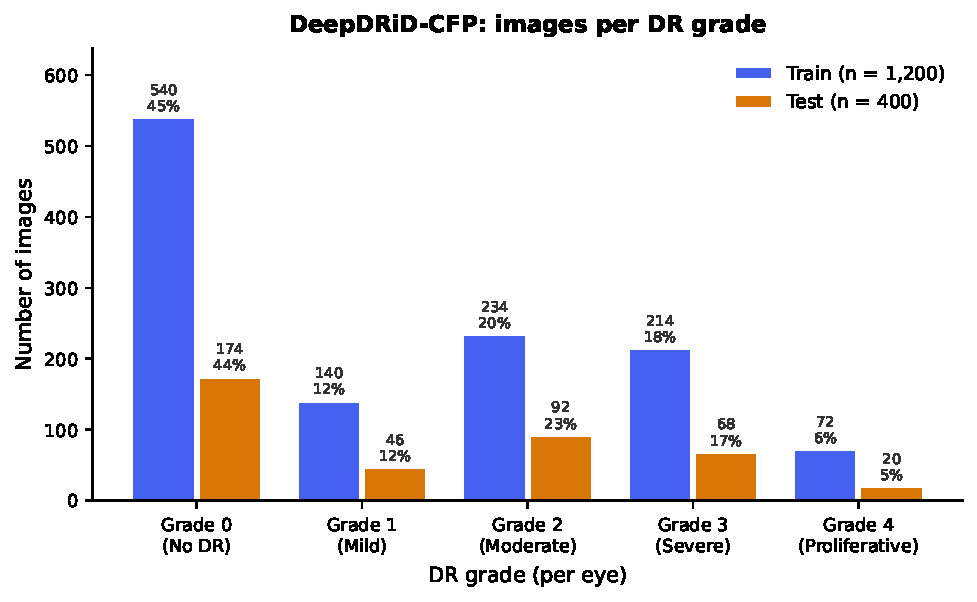
\includegraphics[width=0.92\linewidth]{dataset_distribution}
\caption[توزیع درجه‌ها در آموزش و آزمون \lr{DeepDRiD}]{توزیع درجه‌ها در مجموعه‌های آموزش و آزمون \lr{DeepDRiD} با برچسب سطح چشم (خروجی \lr{notebook} \lr{DeepDRiD\_FewShot\_DR\_fixed}). نسبت درجه‌ها در دو بخش تقریباً یکسان است و درجهٔ ۴ با ۶ درصد \lr{few-shot}‌ترین درجه است.}
\label{fig:dist}
\end{figure}


در \lr{regime} \lr{$k$-shot}، از هر درجه $k$ تصویر آموزشی به‌عنوان \lr{support set} برداشته می‌شود و مقدارهای ۱، ۲، ۴، ۸، ۱۶ و ۳۲ برای $k$ بررسی می‌شوند. هر آزمایش با سه \lr{seed} تصادفی تکرار و میانگین و \lr{standard deviation} گزارش می‌شود. سه نکتهٔ طراحی، نتیجه را منصفانه نگه می‌دارد:
\begin{enumerate}[label=\arabic*.]
\item \textbf{\lr{support}های تودرتو.} \lr{support} \lr{8-shot} همهٔ تصاویر \lr{support} \lr{4-shot} را در بر دارد، پس منحنی عملکرد بر حسب $k$ کمتر \lr{noise} دارد.
\item \textbf{\lr{query} جدا در سطح بیمار.} \lr{query set} که برای \lr{early stopping} و انتخاب \lr{checkpoint} به کار می‌رود، فقط شامل بیمارانی است که هیچ تصویری در \lr{support} ندارند؛ چون هر بیمار چهار تصویر دارد، بدون این \lr{constraint} تصویر چشم دیگر همان بیمار وارد ارزیابی می‌شد.
\item \textbf{پوشش بیماران متفاوت.} در هنگام انتخاب تصاویر \lr{support}، تصاویر بیماران تکراری در اولویت آخر قرار می‌گیرند تا \lr{support} تا حد ممکن بیماران متفاوت را پوشش دهد.
\end{enumerate}

دو حالت مرزی هم ارزیابی می‌شود. در حالت \lr{zero-shot} ($k=0$) هیچ آموزشی انجام نمی‌شود و مدل با وزن‌های اولیه آزموده می‌شود. در حالت \lr{full data} ($k=-1$) کل \lr{training set} استفاده می‌شود، جز ۲۰ درصد بیماران (۶۰ بیمار، ۲۴۰ تصویر) که برای \lr{validation} کنار گذاشته می‌شوند؛ این \lr{holdout} بر اساس بیمار و به تفکیک بدترین درجهٔ هر بیمار انجام می‌شود. \lr{test set} در هیچ حالتی برای انتخاب مدل استفاده نمی‌شود.

\subsubsection{راهبرد تقسیم برای هر \lr{regime}}
\label{sec:split-per-k}
تقسیم هر \lr{regime} از سه مرحلهٔ ثابت ساخته می‌شود و همهٔ آن‌ها در سطح بیمار انجام می‌شوند:
\begin{enumerate}[label=\arabic*.]
\item \textbf{ترتیب نمونه‌گیری هر درجه.} برای هر درجه و هر \lr{seed}، تصاویر آموزشی آن درجه یک بار با مولد تصادفیِ وابسته به (\lr{seed}، درجه) مرتب می‌شوند. در این ترتیب، اولین تصویر هر بیمار پیش از تصویر دوم هر بیماری می‌آید؛ پس تا وقتی بیمار تازه‌ای در آن درجه باقی است، تصویر تکراری از یک بیمار انتخاب نمی‌شود.
\item \textbf{\lr{support}.} \lr{support} \lr{$k$-shot} همان $k$ تصویر اول این ترتیب در هر درجه است، یعنی $5k$ تصویر. چون ترتیب به $k$ وابسته نیست، \lr{support}ها تودرتو هستند و برای هر سه \lr{seed} بررسی شده است که \lr{support} هر $k$ زیرمجموعهٔ \lr{support} $2k$ است.
\item \textbf{\lr{query}.} همهٔ تصاویرِ بیمارانی که حتی یک تصویر در \lr{support} دارند از \lr{query} حذف می‌شوند و بقیهٔ تصاویر آموزش، \lr{query} را می‌سازند. به همین دلیل اندازهٔ \lr{query} از $1200-5k$ کمتر است: هر بیمار \lr{support} چهار تصویرش را از \lr{query} بیرون می‌برد.
\end{enumerate}
\lr{test set} (۴۰۰ تصویر از ۱۰۰ بیمار) در همهٔ \lr{regime}ها یکسان است و فقط یک بار، با بهترین \lr{checkpoint}، ارزیابی می‌شود. جدول~\ref{tab:split-per-k} اندازهٔ هر بخش را برای همهٔ \lr{regime}ها نشان می‌دهد؛ اعداد از فایل‌های تقسیم واقعی شمرده شده‌اند و جایی که بین سه \lr{seed} تفاوت دارند، بازهٔ آن‌ها آمده است.

\begin{table}[H]
\caption{اندازهٔ بخش‌های داده در هر \lr{regime} (سه \lr{seed})}
\label{tab:split-per-k}
\centering\small
\begin{tabular}{@{}lccccc@{}}
\toprule
\textbf{\lr{regime}} & \textbf{تصاویر آموزش} & \textbf{بیماران آموزش} & \textbf{تصاویر \lr{validation}} & \textbf{بیماران \lr{validation}} & \textbf{نقش \lr{validation}}\\
\midrule
\lr{zero-shot} ($k=0$) & -- & -- & -- & -- & بدون آموزش\\
$k=1$ & ۵ & ۵ & \LRE{۱٬۱۸۰} & ۲۹۵ & \lr{query}\\
$k=2$ & ۱۰ & ۱۰ & \LRE{۱٬۱۶۰} & ۲۹۰ & \lr{query}\\
$k=4$ & ۲۰ & ۲۰ & \LRE{۱٬۱۲۰} & ۲۸۰ & \lr{query}\\
$k=8$ & ۴۰ & ۳۹ & \LRE{۱٬۰۴۴} & ۲۶۱ & \lr{query}\\
$k=16$ & ۸۰ & ۷۶ تا ۷۸ & ۸۸۸ تا ۸۹۶ & ۲۲۲ تا ۲۲۴ & \lr{query}\\
$k=32$ & ۱۶۰ & ۱۴۱ تا ۱۴۵ & ۶۲۰ تا ۶۳۶ & ۱۵۵ تا ۱۵۹ & \lr{query}\\
\lr{full data} ($k=-1$) & ۹۶۰ & ۲۴۰ & ۲۴۰ & ۶۰ & \lr{holdout} ۲۰٪ بیماران\\
\bottomrule
\end{tabular}
\end{table}

نکته‌های هر \lr{regime}:
\begin{itemize}
\item \textbf{\lr{zero-shot}.} هیچ تصویر آموزشی دیده نمی‌شود و مدل با \lr{prompt} اولیه روی ۴۰۰ تصویر آزمون سنجیده می‌شود. این \lr{regime} سهم دانش اولیهٔ \lr{CLIP} را جدا می‌کند.
\item \textbf{۱ تا ۴ نمونه.} همهٔ تصاویر \lr{support} از بیماران متفاوت‌اند (۵، ۱۰ و ۲۰ بیمار) و \lr{query} تقریباً کل بقیهٔ دادهٔ آموزش است. در این \lr{regime}ها \lr{SMS} در \lr{1-shot} اثری ندارد، چون \lr{variance} هر درجه صفر است.
\item \textbf{۸ و ۱۶ نمونه.} درون هر درجه همهٔ تصاویر \lr{support} از بیماران متفاوت‌اند، اما یک بیمار ممکن است با یک چشم در یک درجه و با چشم دیگر در درجهٔ دیگری انتخاب شود؛ به همین دلیل تعداد بیماران \lr{support} (۳۹ و ۷۶ تا ۷۸) کمی کمتر از $5k$ است.
\item \textbf{۳۲ نمونه.} \lr{support} ۱۶۰ تصویر از ۱۴۱ تا ۱۴۵ بیمار دارد و ۳۲ تصویر از ۷۲ تصویر درجهٔ ۴ (از ۳۰ بیمار) را مصرف می‌کند؛ \lr{query} به ۶۲۰ تا ۶۳۶ تصویر کاهش می‌یابد ولی هنوز همهٔ درجه‌ها را پوشش می‌دهد.
\item \textbf{\lr{full data}.} به‌جای \lr{support} و \lr{query}، ۲۰ درصد بیماران هر لایه (بیماران با بدترین درجهٔ یکسان) با \lr{seed} اجرا کنار گذاشته می‌شوند: ۹۶۰ تصویر از ۲۴۰ بیمار برای آموزش و ۲۴۰ تصویر از ۶۰ بیمار برای \lr{validation}.
\end{itemize}
\lr{seed}ها \lr{support}های تقریباً جدا از هم می‌سازند (برای نمونه \lr{support} \lr{8-shot} \lr{seed} ۱ و ۲ فقط یک تصویر مشترک دارند)، پس \lr{standard deviation} سه \lr{seed} تغییرپذیری انتخاب \lr{support} را نشان می‌دهد.


\begin{figure}[H]
\begin{diagram}
  \node[datan=6.5cm] (a) {DeepDRiD · 1{,}600 images · 400 patients\\ label = per-eye grade};
  \node[datan=4.2cm,below right=9mm and -22mm of a] (t) {Train: 300 patients · 1{,}200 images};
  \node[datan=4.2cm,below left=9mm and -22mm of a] (x) {Test: 100 patients · 400 images\\ held out for final report only};
  \node[box=3.6cm,below=12mm of t] (k) {$k$-shot: $k$ images per grade\\ nested supports, 3 seeds};
  \node[box=3cm,right=5mm of k] (z) {Zero-shot:\\ no training};
  \node[box=3.2cm,left=5mm of k] (f) {Full data:\\ 80\% patients for training};
  \node[train=3.2cm,below right=9mm and -18mm of k] (ks) {Support $\rightarrow$ training};
  \node[lossn=3.6cm,below left=9mm and -18mm of k] (kq) {Query: patients outside support $\rightarrow$ early stopping};
  \node[lossn=3.2cm,below=26mm of f] (fv) {20\% patients $\rightarrow$ validation};
  \draw[arr] (a)--(t); \draw[arr] (a)--(x);
  \draw[arr] (t)--(k); \draw[arr] (t.south) -- ++(0,-4mm) -| (z.north); \draw[arr] (t.south) -- ++(0,-4mm) -| (f.north);
  \draw[arr] (k)--(ks); \draw[arr] (k)--(kq); \draw[arr] (f)--(fv);
\end{diagram}
\caption{تقسیم داده. همهٔ تقسیم‌ها در سطح بیمار انجام می‌شوند تا هیچ بیماری هم‌زمان در آموزش و ارزیابی نباشد.}
\label{fig:splits}
\end{figure}

% ------------------------------------------------------------------
\subsection{\lr{preprocessing} و \lr{data augmentation}}
در آموزش، ضلع کوتاه‌تر تصویر با \lr{interpolation} \lr{bicubic} به ۲۵۶ پیکسل می‌رسد، سپس برشی تصادفی به اندازهٔ $224\times224$، \lr{random horizontal flip} و \lr{slight colour jitter} (روشنایی، کنتراست و اشباع، هر کدام تا \LRE{۰٫۱}) اعمال و تصویر با میانگین و \lr{standard deviation} \lr{CLIP} نرمال می‌شود. در ارزیابی به‌جای \lr{random crop}، \lr{centre crop} به کار می‌رود و \lr{data augmentation}‌ای در کار نیست. \lr{preprocessing} \lr{baseline}ها در دستور رسمی خودشان (تغییر اندازه به مربع ۲۵۶، برش، \lr{flipping} و \lr{normalisation} \lr{ImageNet}) فقط در \lr{configuration}های «\lr{official}» استفاده می‌شود.

\begin{figure}[H]
\begin{diagram}
  \node[datan=2.4cm] (i) {Raw Image};
  \node[box=2.6cm,right=6mm of i] (r) {Resize short side to 256 (bicubic)};
  \node[train=2.4cm,right=6mm of r] (c) {Random crop $224^2$};
  \node[train=2.4cm,right=6mm of c] (h) {H-flip + colour jitter 0.1};
  \node[box=2.4cm,right=6mm of h] (n) {CLIP normalise};
  \node[box=2.4cm,below=9mm of c] (cc) {Centre crop $224^2$};
  \draw[arr] (i)--(r); \draw[arr] (r)--(c); \draw[arr] (c)--(h); \draw[arr] (h)--(n);
  \draw[darr] (r.south) |- (cc.west); \draw[darr] (cc.east) -| (n.south);
  \node[elabel,above=1mm of c] {Train};
  \node[elabel,below=1mm of cc] {Eval};
\end{diagram}
\caption{زنجیرهٔ \lr{preprocessing}. مسیر پیوسته در آموزش و مسیر خط‌چین در ارزیابی به کار می‌رود.}
\label{fig:preproc}
\end{figure}

% ------------------------------------------------------------------
\subsection{معماری و \lr{block}های مدل}
\begin{figure}[H]
\begin{diagram}
  % Coordinates for branch column centers
  \coordinate (tc) at (-3.8, 0);
  \coordinate (ic) at (3.8, 0);

  % --- Text branch (left) ---
  \node[train=2.8cm] (c) at ($(tc) + (-1.55, 0)$) {16 shared context\\ tokens $c_1\dots c_{16}$};
  \node[train=2.8cm] (b) at ($(tc) + (1.55, 0)$) {3 base rank\\ tokens $\beta$};
  \node[box=2.8cm,below=6mm of b] (i) {OrdinalCLIP interp.\\ $\rightarrow$ 5 rank tokens $r_0\dots r_4$};
  \node[box=5.6cm,anchor=north] (pr) at ($(tc |- i.south) + (0,-7mm)$) {Prompt for grade $k$:\\ {[SOS]} $c_1\dots c_{16}\ r_k$ [EOS]};
  \node[frozen=5.6cm,below=6mm of pr] (te) {CLIP text encoder (frozen)};
  \node[box=5.6cm,below=6mm of te] (t) {$t_0\dots t_4$: grade prototypes};

  % --- Image branch (right) ---
  \node[datan=3.8cm,anchor=north] (x) at (ic |- b.north) {Fundus Image\\ $224\times224$};
  \node[box=3.8cm,anchor=south] (z) at (ic |- t.south) {$z$: 1024-d image vector\\ normalised};
  \node[train=3.8cm] (v) at ($(x.south)!0.5!(z.north)$) {CLIP RN50 Image Encoder\\ frozen + LoRA on convolutions};

  % --- Joint stage (centered) ---
  \node[box=5.0cm,below=9mm of $(t.south)!0.5!(z.south)$] (s) {Similarity matrix\\ $s = 100\cdot z\,t^{\top}$};

  % --- Downstream outputs ---
  \node[box=3.8cm,below left=8mm and 2mm of s.south] (p) {Prediction:\\ softmax \& argmax};
  \node[box=4.0cm,below right=8mm and 2mm of s.south] (sms) {SMS: statistical calibration\\ (train only)};
  \node[lossn=4.0cm,below=6mm of sms] (l) {Cross-entropy +\\ rank-aware loss};

  % --- Connections ---
  \draw[arr] (x) -- (v);
  \draw[arr] (v) -- (z);
  \draw[arr] (b) -- (i);
  \draw[arr] (c.south) -- (pr.north -| c.south);
  \draw[arr] (i.south) -- (pr.north -| i.south);
  \draw[arr] (pr) -- (te);
  \draw[arr] (te) -- (t);
  \draw[arr] (t.south) |- (s.west);
  \draw[arr] (z.south) |- (s.east);
  \draw[arr] (s) -- (p);
  \draw[arr] (s) -- (sms);
  \draw[arr] (sms) -- (l);

  % --- Groups ---
  \begin{scope}[on background layer]
    \node[group,fit=(x)(v)(z)] (gi) {};
    \node[group,fit=(b)(c)(i)(pr)(te)(t)] (gt) {};
  \end{scope}
  \node[grouplabel,anchor=south] at (gi.north) {Image branch};
  \node[grouplabel,anchor=south] at (gt.north) {Text branch};
\end{diagram}
\archlegend
\caption{معماری مدل پایه. \lr{block}های \lr{frozen} \lr{CLIP} تغییر نمی‌کنند؛ فقط ماتریس‌های \lr{LoRA}، \lr{context token}ها و سه \lr{base rank token} آموخته می‌شوند.}
\label{fig:m-arch}
\end{figure}

\subsubsection{\lr{image branch}: \lr{CLIP RN50} با \lr{LoRA}}
\lr{image encoder}، شبکهٔ \lr{ResNet-50} مدل \lr{CLIP} است که بردار ۱۰۲۴-بعدی تولید می‌کند. وزن‌های آن \lr{frozen} می‌مانند و روی همهٔ لایه‌های \lr{convolution} (لایه‌های ورودی و سه \lr{convolution} هر \lr{bottleneck block}) \lr{low-rank adaptation} (\lr{LoRA} \cite{lora}) اضافه می‌شود. این روش به‌جای تغییر وزن $W$، حاصل‌ضرب دو ماتریس کوچک را به آن می‌افزاید:
\begin{equation}
W' = W + \frac{\alpha}{r}\, B A, \qquad r = 16,\ \alpha = 16,\ B_{\text{init}} = 0
\label{eq:lora}
\end{equation}
با $B=0$ در آغاز، مدل دقیقاً همان \lr{CLIP} اولیه است. \lr{dropout} \lr{LoRA} برابر \LRE{۰٫۱} است و کل \lr{parameter}های آن \LRE{۱٬۱۸۸٬۲۷۲} است. خروجی \lr{encoder} به طول واحد نرمال می‌شود: $z = f_\theta(x) / \lVert f_\theta(x) \rVert$.

\begin{figure}[H]
\begin{diagram}
  \node[datan=1.4cm] (in) at (0,0) {$x$};
  \node[frozen=3.4cm] (w) at (4.8,1.1) {$W$ frozen (main convolution)};
  \node[train=1.5cm] (a) at (2.6,-1.1) {$A$\\ $r=16$};
  \node[train=1.7cm] (bb) at (4.8,-1.1) {$B$\\ init: zero};
  \node[box=1.3cm] (sc) at (7.0,-1.1) {$\times\,\alpha/r$};
  \node[circle,draw=navy,thick,inner sep=1pt] (plus) at (8.7,0) {$+$};
  \node[datan=1.6cm] (out) at (10.2,0) {$W'x$};
  \draw[arr] (in.east) -- (1.2,0) |- (w.west);
  \draw[arr] (1.2,0) |- (a.west);
  \draw[arr] (a)--(bb); \draw[arr] (bb)--(sc);
  \draw[arr] (w.east) -| (plus.north);
  \draw[arr] (sc.east) -| (plus.south);
  \draw[arr] (plus)--(out);
  \fill[navy!80] (1.2,0) circle (1.2pt);
\end{diagram}
\caption{\lr{block} \lr{LoRA} روی هر لایهٔ \lr{convolution} (رابطهٔ~\ref{eq:lora}). مسیر بالا \lr{frozen} است و فقط $A$ و $B$ آموخته می‌شوند.}
\label{fig:lora}
\end{figure}

\subsubsection{\lr{text branch}: \lr{prompt} رتبه‌ای با \lr{interpolation} \lr{OrdinalCLIP}}
برای هر درجهٔ $k$ یک دنبالهٔ توکن ساخته می‌شود: نشانهٔ آغاز، ۱۶ \lr{context token} مشترک $c_1,\dots,c_{16}$، یک \lr{rank token} $r_k$ و نشانهٔ پایان. \lr{context token}ها بین همهٔ درجه‌ها مشترک‌اند و با توزیع نرمال با \lr{standard deviation} \LRE{۰٫۰۲} آغاز می‌شوند. \lr{rank token}ها آزاد نیستند: از سه بردار پایهٔ \lr{learnable} $\beta_0,\beta_1,\beta_2$ که در موقعیت‌های $\pi=(0,2,4)$ روی محور درجه قرار گرفته‌اند، با وزن‌دهی خطی \lr{OrdinalCLIP} ساخته می‌شوند:
\begin{equation}
r_k = \sum_{b=0}^{2} W_{kb}\, \beta_b, \qquad W_{kb} = \frac{1 - |k - \pi_b|/(K-1)}{\sum_{b'} \big(1 - |k - \pi_{b'}|/(K-1)\big)}
\label{eq:interp}
\end{equation}
در این وزن‌دهی هر درجه آمیزه‌ای از هر سه پایه است، نه فقط دو پایهٔ نزدیک؛ بنابراین درجه‌های مجاور توکن‌های شبیه به هم دارند و ترتیب در خود \lr{parameterisation} نهفته است. این وزن‌ها با کد رسمی \lr{OrdinalCLIP} مقایسه و یکسان یافته شده‌اند.

\begin{table}[H]
\caption{ماتریس وزن \lr{interpolation} $W$ برای ۵ درجه و ۳ پایه}
\label{tab:interp}
\centering
\begin{tabular}{@{}cccc@{}}
\toprule
\textbf{درجه} & $\beta_0$ & $\beta_1$ & $\beta_2$\\
\midrule
۰ & \LRE{۰٫۶۶۷} & \LRE{۰٫۳۳۳} & ۰\\
۱ & \LRE{۰٫۴۲۹} & \LRE{۰٫۴۲۹} & \LRE{۰٫۱۴۳}\\
۲ & \LRE{۰٫۲۵۰} & \LRE{۰٫۵۰۰} & \LRE{۰٫۲۵۰}\\
۳ & \LRE{۰٫۱۴۳} & \LRE{۰٫۴۲۹} & \LRE{۰٫۴۲۹}\\
۴ & ۰ & \LRE{۰٫۳۳۳} & \LRE{۰٫۶۶۷}\\
\bottomrule
\end{tabular}
\end{table}

دنبالهٔ هر درجه از \lr{text encoder} \lr{frozen} \lr{CLIP} (\lr{Transformer} ۱۲ لایه با پهنای ۵۱۲) عبور می‌کند و خروجیِ موقعیت نشانهٔ پایان پس از تصویر خطی، \lr{prototype} آن درجه است: $t_k = g(p_k) / \lVert g(p_k) \rVert$. \lr{parameter}های \lr{trainable} این شاخه $16\times512$ برای بافت و $3\times512$ برای پایه‌ها، در مجموع \LRE{۹٬۷۲۸} است.

\begin{figure}[H]
\begin{diagram}[x=-1.15cm]
  \foreach \i/\n in {0/0,2/2,4/4} \node[train=1.3cm] (beta\i) at (-2*\i,0) {$\beta_{\pgfmathparse{int(\i/2)}\pgfmathresult}$\\ \footnotesize pos.~\n};
  \foreach \k/\n in {0/0,1/1,2/2,3/3,4/4} \node[box=1.3cm] (r\k) at (-2*\k,-2.4) {$r_\k$\\ \footnotesize grade~\n};
  \foreach \k in {0,...,4} \foreach \i in {0,2,4} \draw[->,draw=navy!35] (beta\i.south) -- (r\k.north);
  \draw[arr,very thick] (beta0.south) -- (r0.north);
  \draw[arr,very thick] (beta2.south) -- (r2.north);
  \draw[arr,very thick] (beta4.south) -- (r4.north);
\end{diagram}
\caption{\lr{interpolation} \lr{rank token}ها (رابطهٔ~\ref{eq:interp}). هر \lr{rank token} ترکیب وزن‌دار هر سه پایه است و وزن پایهٔ نزدیک‌تر بیشتر است (جدول~\ref{tab:interp}).}
\label{fig:interp}
\end{figure}

\subsubsection{\lr{similarity matrix} و پیش‌بینی}
\lr{similarity} تصویر $b$ با درجهٔ $k$ ضرب داخلی دو بردار نرمال‌شده در \lr{logit scale} \lr{CLIP} است. این مقیاس در مقدار ۱۰۰ ثابت نگه داشته می‌شود، همان‌طور که در \lr{OrdinalCLIP} و \lr{CLIP-DR}:
\begin{equation}
s_{bk} = \tau^{-1}\, z_b^{\top} t_k, \qquad \tau^{-1} = 100, \qquad p_{bk} = \frac{\exp(s_{bk})}{\sum_{j} \exp(s_{bj})}, \qquad \hat{y}_b = \arg\max_k p_{bk}
\label{eq:sim}
\end{equation}

\subsubsection{\lr{Similarity Matrix Smoothing} (\lr{SMS})}
\label{sec:sms}
این جزء از \lr{CLIP-DR} \cite{clipdr} گرفته شده و صورت دقیق آن \lr{Feature Distribution Smoothing} (\lr{FDS} \cite{fds}) است که روی بردار ۵-بعدی \lr{similarity} هر تصویر اجرا می‌شود. ایده این است که \lr{similarity statistic} تصاویر یک درجه نباید از درجه‌های همسایه‌اش فاصلهٔ زیادی داشته باشد. برای هر درجهٔ $j$، در طول یک \lr{epoch} میانگین $\mu_j$ و \lr{variance} $\Sigma_j$ بردارهای \lr{similarity} تصاویر آن درجه، به تفکیک هر بُعد، جمع‌آوری می‌شود. این \lr{statistic}ها با \lr{momentum} $m=0.9$ بین \lr{epoch}ها به‌روزرسانی و سپس با \lr{Gaussian kernel} روی محور درجه هموار می‌شوند:
\begin{equation}
\tilde{\mu}_j = \sum_{j'} g(j - j')\, \mu_{j'}, \qquad \tilde{\Sigma}_j = \sum_{j'} g(j - j')\, \Sigma_{j'}, \qquad g = (0.186,\ 0.205,\ 0.217,\ 0.205,\ 0.186)
\end{equation}
\lr{kernel} اندازهٔ ۵ و \lr{standard deviation} ۲ دارد و در لبه‌های محور درجه، بازتابی گسترش می‌یابد. در \lr{epoch} بعد، \lr{similarity} هر تصویر آموزشی با \lr{statistic} درجهٔ خودش بازمقیاس می‌شود و \lr{loss} روی همین \lr{similarity} \lr{calibrated} محاسبه می‌شود:
\begin{equation}
\tilde{s}_b = \big(s_b - \mu_{y_b}\big) \odot \sqrt{\operatorname{clip}\!\big(\tilde{\Sigma}_{y_b} / \Sigma_{y_b},\ 0.5,\ 2\big)} + \tilde{\mu}_{y_b}
\label{eq:sms}
\end{equation}
چون این \lr{calibration} به درجهٔ واقعی نیاز دارد، فقط در آموزش اعمال می‌شود و در آزمون \lr{similarity} خام به کار می‌رود. در حالت \lr{1-shot}، هر درجه در هر \lr{epoch} فقط یک تصویر دارد و \lr{variance} صفر است؛ در این حالت \lr{SMS} عملاً هیچ اثری ندارد.

\begin{notebox}[نکته برای گزارش.]
در کد منتشرشدهٔ \lr{CLIP-DR} فراخوانی‌های \lr{SMS} غیرفعال (توضیح‌کد) شده‌اند، هرچند مقاله اثر آن را گزارش می‌کند. به همین دلیل نسخهٔ \lr{matched} \lr{CLIP-DR} در این پژوهش بدون \lr{SMS} اجرا می‌شود.
\end{notebox}

\begin{figure}[H]
\begin{diagram}
  \node[datan=3cm] (a) {Epoch $e$: each batch};
  \node[box=3cm,below=of a] (b) {Raw similarity $s$};
  \node[box=3.6cm,below right=9mm and -10mm of b] (c) {Accumulate stats: mean \& variance per grade};
  \node[train=3.6cm,below left=9mm and -10mm of b] (d) {Calibrate with epoch $e{-}1$ stats, Eq.~\ref{eq:sms}};
  \node[lossn=3.6cm,below=of d] (e) {Loss \& gradients};
  \node[box=3.6cm,below=of c] (f) {End of epoch: momentum 0.9 + Gaussian smooth over grades};
  \node[datan=3.6cm,below=of f] (g) {Fixed stats for epoch $e{+}1$};
  \draw[arr] (a)--(b); \draw[arr] (b)--(c); \draw[arr] (b)--(d); \draw[arr] (d)--(e); \draw[arr] (c)--(f); \draw[arr] (f)--(g);
  \draw[darr] (g.west) -| ([xshift=-14mm]d.west) -- (d.west);
\end{diagram}
\caption{چرخهٔ \lr{SMS} در هر \lr{epoch}. \lr{statistic}ها در طول \lr{epoch} ثابت‌اند و فقط در پایان \lr{epoch} به‌روز می‌شوند.}
\label{fig:sms}
\end{figure}

% ------------------------------------------------------------------
\subsection{\lr{loss function}ها}
\lr{loss} کل مدل پایه دو جزء دارد که هر دو روی \lr{similarity} \lr{calibrated} $\tilde{s}$ محاسبه می‌شوند:
\begin{equation}
\mathcal{L} = \mathcal{L}_{\mathrm{CE}}(\tilde{s}, y) + \lambda_{\mathrm{rank}}\, \mathcal{L}_{\mathrm{rank}}(\tilde{s}, y), \qquad \lambda_{\mathrm{rank}} = 1
\label{eq:m-loss}
\end{equation}

\paragraph{\lr{cross-entropy}.} \lr{loss} استاندارد طبقه‌بندی که تصویر را به \lr{prototype} درجهٔ درست نزدیک و از بقیه دور می‌کند: $\mathcal{L}_{\mathrm{CE}} = -\frac{1}{B} \sum_b \log p_{b, y_b}$. این \lr{loss} به تنهایی ترتیب را نمی‌بیند؛ پیش‌بینی درجهٔ ۴ برای تصویر درجهٔ ۰ همان‌قدر جریمه می‌شود که پیش‌بینی درجهٔ ۱.

\paragraph{\lr{ranking-aware loss}.} این \lr{loss} از \lr{CLIP-DR} است و شکل «\lr{unimodal}» را تحمیل می‌کند: \lr{similarity} تصویر با درجه‌ها باید از درجهٔ درست به سمت هر دو طرف به‌طور یکنواخت کاهش یابد. برای هر جفت درجهٔ مجاور در سمت راست و چپ درجهٔ درست، \lr{pairwise loss} \lr{logistic} اعمال می‌شود:
\begin{equation}
\mathcal{L}_{\mathrm{rank}} = \frac{1}{B} \sum_{b} \Bigg[ \sum_{r = y_b}^{K-2} -\log \sigma\!\Big(\frac{s_{b,r} - s_{b,r+1}}{\tau_r}\Big) + \sum_{r = 1}^{y_b} -\log \sigma\!\Big(\frac{s_{b,r} - s_{b,r-1}}{\tau_r}\Big) \Bigg], \qquad \tau_r = 1
\label{eq:rank}
\end{equation}
این صورت همان رابطهٔ مقاله است. کد \lr{CLIP-DR} همین \lr{constraint} را با \lr{cross-entropy} روی بردارهایی پیاده می‌کند که درایه‌های غیرمرتبطشان صفر است و فقط سه گام فاصله را می‌پوشاند؛ صورت بالا همهٔ جفت‌ها را بدون آن درایه‌های صفر در بر دارد.

\begin{figure}[H]
\centering
\begin{latin}
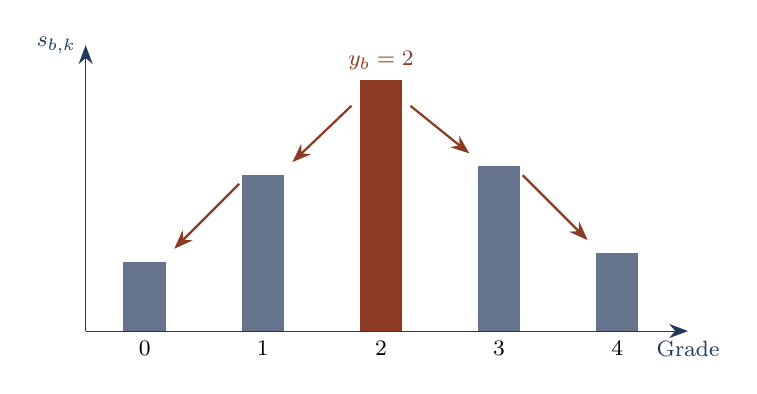
\begin{tikzpicture}[x=1.5cm,y=1.1cm]
  \draw[->,navy] (-0.5,0) -- (4.6,0) node[below,font=\footnotesize] {Grade};
  \draw[->,navy] (-0.5,0) -- (-0.5,3.3) node[left,font=\footnotesize] {$s_{b,k}$};
  \foreach \k/\n in {0/0,1/1,2/2,3/3,4/4} \node[below,font=\footnotesize] at (\k,0) {\n};
  \foreach \k/\h in {0/0.8,1/1.8,2/2.9,3/1.9,4/0.9} \fill[navy!70] (\k-0.18,0) rectangle (\k+0.18,\h);
  \fill[accent] (2-0.18,0) rectangle (2+0.18,2.9);
  \node[above,font=\footnotesize,accent] at (2,2.9) {$y_b=2$};
  \draw[->,thick,accent] (1.75,2.6) -- (1.25,1.95);
  \draw[->,thick,accent] (2.25,2.6) -- (2.75,2.05);
  \draw[->,thick,accent] (0.8,1.7) -- (0.25,0.95);
  \draw[->,thick,accent] (3.2,1.8) -- (3.75,1.05);
\end{tikzpicture}
\end{latin}
\caption{شکل \lr{unimodal} که \lr{ranking-aware loss} (رابطهٔ~\ref{eq:rank}) تحمیل می‌کند: هر پیکان یک جملهٔ \lr{pairwise loss} است که \lr{similarity} درجهٔ نزدیک‌تر را از درجهٔ دورتر بیشتر می‌خواهد.}
\label{fig:rank}
\end{figure}

\begin{notebox}[اجزای کنارگذاشته‌شده.]
\lr{RankFormer} و \lr{distance-weighted pairwise loss}، که از مقالهٔ \lr{L2RCLIP} \cite{l2rclip} الهام گرفته‌اند، جزو مدل پایه نیستند. \lr{repository} رسمی \lr{L2RCLIP} کد مدل، کد آموزش و وزن‌های آموخته را منتشر نکرده است، پس درستی پیاده‌سازی را فقط می‌توان با متن مقاله سنجید. این دو جزء به‌صورت \lr{configuration}های جداگانه نگه داشته شده‌اند و در بخش~\ref{sec:m-baselines} شرح داده می‌شوند.
\end{notebox}

% ------------------------------------------------------------------
\subsection{آموزش و بهینه‌سازی}
\begin{table}[H]
\caption{تنظیمات آموزش مدل پایه}
\label{tab:train}
\centering
\begin{tabularx}{0.92\textwidth}{@{}l X@{}}
\toprule
\textbf{مؤلفه} & \textbf{مقدار}\\
\midrule
\lr{optimizer} & \lr{AdamW}، \lr{learning rate} $10^{-4}$، \lr{weight decay} $10^{-4}$\\
\lr{schedule} \lr{learning rate} & ۵ \lr{epoch} \lr{linear warm-up} و سپس \lr{cosine decay}\\
تعداد \lr{epoch} & ۵۰ (یکسان برای همهٔ مدل‌های \lr{matched})\\
\lr{batch size} & آموزش: کمینهٔ اندازهٔ \lr{support} و ۳۲؛ ارزیابی: ۳۲\\
\lr{early stopping} & صبر ۲۰ \lr{epoch} روی \lr{QWK} \lr{query set}\\
\lr{checkpoint}ها & بهترین مدل بر اساس \lr{QWK} \lr{query} و آخرین \lr{epoch}، پس از هر \lr{epoch}؛ آزمون با بهترین\\
دقت عددی و پایداری & آمیختهٔ \lr{bf16}، \lr{gradient clipping} با نُرم ۱\\
\lr{parameter}های \lr{frozen} & همهٔ \lr{CLIP}، از جمله \lr{token embedding table} و \lr{logit scale}\\
\lr{parameter}های \lr{trainable} & \lr{LoRA} تصویر \LRE{۱٬۱۸۸٬۲۷۲} + توکن‌ها \LRE{۹٬۷۲۸} = \LRE{۱٬۱۹۸٬۰۰۰}\\
\bottomrule
\end{tabularx}
\end{table}

\begin{figure}[H]
\begin{diagram}
  \node[datan=4.6cm] (s) {Start run: config + $k$ + seed};
  \node[decision,below=of s] (c) {Already run?};
  \node[datan=3.4cm,left=14mm of c] (r) {Load result from shared cache};
  \node[train=4cm,below=of c] (e) {One training epoch on support};
  \node[box=4cm,below=of e] (v) {Validate on query: QWK \& metrics};
  \node[box=4cm,below=of v] (k) {Save \texttt{best} and \texttt{last}};
  \node[decision,below=of k] (d) {Improved in 20 epochs\\ and epoch $<50$?};
  \node[box=4cm,below=of d] (b) {Load best checkpoint};
  \node[lossn=4cm,below=of b] (t) {Test on 400 images};
  \node[datan=4cm,below=of t] (m) {Save metrics and confusion matrix};
  \draw[arr] (s)--(c); \draw[arr] (c)--node[elabel,above]{yes}(r); \draw[arr] (c)--node[elabel,right]{no}(e);
  \draw[arr] (e)--(v); \draw[arr] (v)--(k); \draw[arr] (k)--(d);
  \draw[arr] (d.east) -- node[elabel,above]{yes} ++(14mm,0) |- (e.east);
  \draw[arr] (d)--node[elabel,right]{no}(b); \draw[arr] (b)--(t); \draw[arr] (t)--(m);
\end{diagram}
\caption{گردش کار یک اجرا. اجرای قطع‌شده از آخرین \lr{checkpoint} ادامه می‌یابد و اجرای تکراری دوباره آموزش داده نمی‌شود.}
\label{fig:run}
\end{figure}

% ------------------------------------------------------------------
\subsection{ارزیابی و \lr{metric}ها}
\label{sec:metrics}
همهٔ \lr{metric}ها روی ۴۰۰ تصویر آزمون و با پیش‌بینی بیشینه‌احتمال محاسبه می‌شوند. \lr{metric} اصلی \lr{QWK} است و دو \lr{metric} ترتیبی \lr{ODC} و \lr{error mass} بر حسب فاصله نشان می‌دهند که آیا خطاها «نزدیک» هستند. سه \lr{metric} \lr{calibration} (\lr{ECE}، \lr{NLL} و \lr{Brier}) کیفیت احتمال‌های پیش‌بینی‌شده را می‌سنجند.

\begin{figure}[H]
\begin{diagram}
  \node[datan=3.6cm] (p) {Predicted probs.~$p_{ik}$ on 400 images};
  \node[box=3cm,below right=9mm and -6mm of p] (cm) {Confusion matrix $O$};
  \node[box=3cm,below left=9mm and -6mm of p] (pr) {Full probability distribution};
  \node[lossn=2.6cm,below right=9mm and -16mm of cm] (g1) {\textbf{Agreement}\\ QWK · MAE · F1 · Acc};
  \node[lossn=2.6cm,below left=9mm and -16mm of cm] (g2) {\textbf{Error shape}\\ ODC · mass by distance};
  \node[lossn=2.6cm,below=9mm of pr] (g3) {\textbf{Calibration}\\ ECE · NLL · Brier};
  \node[lossn=2.2cm,left=4mm of g3] (g4) {\textbf{Ranking}\\ AUC · LOS};
  \draw[arr] (p)--(cm); \draw[arr] (p)--(pr); \draw[arr] (cm)--(g1); \draw[arr] (cm)--(g2); \draw[arr] (pr)--(g3); \draw[arr] (pr)--(g4);
\end{diagram}
\caption{چهار گروه \lr{metric} و ورودی هر گروه.}
\label{fig:metrics}
\end{figure}

\paragraph{\lr{Quadratic Weighted Kappa} (\lr{QWK}).} توافق پیش‌بینی و برچسب، با جریمه‌ای متناسب با مجذور فاصلهٔ درجه‌ها. $O$ \lr{confusion matrix} و $E$ ماتریس مورد انتظار تحت استقلال است:
\begin{equation}
\kappa_w = 1 - \frac{\sum_{i,j} w_{ij} O_{ij}}{\sum_{i,j} w_{ij} E_{ij}}, \qquad w_{ij} = \frac{(i - j)^2}{(K-1)^2}
\end{equation}

\paragraph{\lr{mean absolute error}، \lr{F1} کلان، دقت و \lr{AUC}.} $\mathrm{MAE} = \frac{1}{N} \sum_i |\hat{y}_i - y_i|$ فاصلهٔ متوسط پیش‌بینی از درجهٔ درست است. \lr{metric} \lr{F1} کلان میانگین \lr{F1} پنج درجه است و به درجه‌های \lr{few-shot} وزن برابر می‌دهد. \lr{area under the curve} (\lr{AUC}) به روش \lr{one-vs-rest} و با \lr{macro average} محاسبه می‌شود؛ \lr{CLIP-DR} در گزارش خود روش \lr{one-vs-one} را به کار برده است و در مقایسه با اعداد آن مقاله باید به این تفاوت توجه کرد.

\paragraph{\lr{local ordinal score} (\lr{LOS}).} سهم تصاویری که احتمال درجهٔ پیش‌بینی‌شده‌شان از هر دو درجهٔ همسایه بیشتر است، یعنی توزیع پیش‌بینی در آن نقطه قله دارد.

\paragraph{\lr{ordinal decay consistency} (\lr{ODC}).} برای هر سطر $i$ از \lr{confusion matrix} که \lr{normalisation} سطری شده ($P_{ij}$)، با حرکت از قطر به سمت دو لبه، مجموع افزایش‌های \lr{error mass} شمرده می‌شود:
\begin{equation}
v_i = \sum_{j > i} \max\!\big(0,\ P_{i,j+1} - P_{i,j}\big) + \sum_{j < i} \max\!\big(0,\ P_{i,j-1} - P_{i,j}\big), \qquad \mathrm{ODC} = 1 - \frac{1}{|\mathcal{I}|} \sum_{i \in \mathcal{I}} v_i
\end{equation}
مجموعهٔ $\mathcal{I}$ سطرهایی است که نمونه دارند. در صورت کامل ($\mathrm{ODC}_{\mathrm{full}}$)، گام از خود قطر هم شمرده می‌شود و در صورت خارج‌قطری ($\mathrm{ODC}_{\mathrm{offdiag}}$) شمارش از یک گام بعد از قطر آغاز می‌شود. مقدار ۱ یعنی در هر سطر \lr{error mass} با دور شدن از قطر هرگز افزایش نمی‌یابد. سهم سطرهایی که هیچ نقض ندارند هم گزارش می‌شود.

\paragraph{\lr{error mass} بر حسب فاصله.} مقدار $m_\Delta$ میانگین سطری جرم پیش‌بینی در فاصلهٔ $|\hat{y} - y| = \Delta$ است، برای $\Delta = 0,\dots,4$. مدل ترتیبی خوب بیشترین جرم را در $\Delta=0$ و جرمی نزولی در فاصله‌های بعدی دارد.

\paragraph{\lr{metric}های \lr{calibration}.} \lr{expected calibration error} (\lr{ECE}) با ۱۵ بازهٔ هم‌عرض اطمینان محاسبه می‌شود. \lr{negative log-likelihood} (\lr{NLL}) و \lr{Brier score} هر دو \lr{proper scoring rules} هستند و کل توزیع احتمال را می‌سنجند:
\begin{equation}
\begin{gathered}
\mathrm{ECE} = \sum_{m=1}^{15} \frac{|B_m|}{N} \big| \mathrm{acc}(B_m) - \mathrm{conf}(B_m) \big|,\\
\mathrm{NLL} = -\frac{1}{N} \sum_i \log p_{i, y_i}, \qquad \mathrm{Brier} = \frac{1}{N} \sum_i \sum_k \big(p_{ik} - \mathbb{1}[y_i = k]\big)^2
\end{gathered}
\end{equation}

% ------------------------------------------------------------------
\subsection{\lr{baseline}ها و \lr{ablation}ها}
\label{sec:m-baselines}
همهٔ \lr{baseline}ها با کد اصلی نویسندگانشان بررسی شده‌اند. برای هر کدام دو نسخه وجود دارد: نسخهٔ «\lr{matched}» که فقط روش را از مقاله می‌گیرد و بقیهٔ شرایط (پشتوانهٔ \lr{RN50}، بودجهٔ آموزش، \lr{preprocessing} و داده) را با مدل ما یکسان نگه می‌دارد، و نسخهٔ «\lr{official}» که دستور آموزش خود نویسندگان را اجرا می‌کند.

\begin{table}[H]
\caption{\lr{baseline}ها در شاخهٔ \lr{master}}
\label{tab:baselines}
\centering\small
\begin{tabularx}{\textwidth}{@{}p{2.6cm} X p{3cm} X@{}}
\toprule
\textbf{مدل} & \textbf{\lr{prompt learner}} & \textbf{\lr{loss}} & \textbf{\lr{image encoder} و آموزش}\\
\midrule
\lr{OrdinalCLIP} \lr{matched} & ۱۳ \lr{context token} آغازشده از جملهٔ متنی، ۳ پایهٔ \lr{interpolation}، نقطهٔ پایان جمله & \lr{CE + KL} & \lr{frozen}؛ تنظیمات ما\\
\lr{OrdinalCLIP} \lr{official} & همان & \lr{CE + KL} & \lr{full fine-tuning}؛ \lr{RAdam}، \lr{weight decay} $5\times10^{-4}$، ۱۰۰ \lr{epoch}، \lr{preprocessing} \lr{ImageNet}\\
\lr{CLIP-DR} \lr{matched} & ۱۰ \lr{context token} تصادفی، ۵ \lr{rank token} آزاد، نقطهٔ پایان جمله & \lr{CE + KL} + \lr{loss} رتبه؛ بدون \lr{SMS} & \lr{LoRA}؛ تنظیمات ما\\
\lr{CLIP-DR} \lr{official} & همان & همان & \lr{full fine-tuning}؛ \lr{RAdam}، بدون \lr{weight decay}، ۳۱ \lr{epoch}، \lr{batch} ۶۴\\
\lr{L2RCLIP} (پیاده‌سازی ما) & \lr{RankFormer} روی \lr{rank token}ها & \lr{CE} + \lr{distance-weighted pairwise loss} & \lr{LoRA}؛ تنظیمات ما؛ بدون \lr{SMS} و \lr{loss} رتبه\\
\bottomrule
\end{tabularx}
\end{table}

\paragraph{\lr{loss} \lr{KL} در \lr{OrdinalCLIP}.} برای هر درجهٔ $k$ که در \lr{batch} حضور دارد، توزیع \lr{similarity} آن درجه روی تصاویر \lr{batch} به توزیعی تقریباً یکنواخت روی تصاویرِ همان درجه نزدیک می‌شود:
\begin{equation}
\mathcal{L}_{\mathrm{KL}} = \frac{1}{|\mathcal{K}_B|} \sum_{k \in \mathcal{K}_B} \mathrm{KL}\!\Big( \operatorname{softmax}_b\!\big(10\, \mathbb{1}[y_b = k]\big) \,\Big\Vert\, \operatorname{softmax}_b\!\big(s_{bk}\big) \Big)
\end{equation}

\paragraph{\lr{block} \lr{RankFormer}.} در پیاده‌سازی ما بر اساس مقالهٔ \lr{L2RCLIP}، \lr{rank token}ها پیش از ورود به \lr{text encoder} از یک \lr{attention block} می‌گذرند: $R' = (1-\alpha) R + \alpha\, \mathrm{FFN}(\mathrm{MSA}(\mathrm{LN}(R)))$ با $\alpha = 0.5$، \lr{multi-head attention} با ۴ سر و \lr{feed-forward network} $512 \to 2048 \to 512$ که لایهٔ خروجی‌اش با صفر آغاز می‌شود. مقدار $\alpha$ در مقاله گزارش نشده و انتخاب ماست.

\paragraph{\lr{distance-weighted pairwise loss}.} این \lr{loss} از ایدهٔ \lr{L2RCLIP} الهام گرفته اما همان \lr{loss} مقاله نیست:
\begin{equation}
\mathcal{L}_{\mathrm{pair}} = \frac{1}{B} \sum_b \sum_{j \ne y_b} |y_b - j| \cdot \big(-\log \sigma(s_{b,y_b} - s_{bj})\big)
\label{eq:pair}
\end{equation}
هرچه درجهٔ اشتباه دورتر باشد، نزدیک بودن تصویر به آن بیشتر جریمه می‌شود.

\begin{table}[H]
\caption{\lr{ablation}ها مدل پایه (هر کدام فقط در یک جزء با مدل کامل تفاوت دارد)}
\label{tab:m-ablation}
\centering\small
\begin{tabularx}{\textwidth}{@{}p{3.4cm} X X@{}}
\toprule
\textbf{آزمایش} & \textbf{تغییر} & \textbf{پرسشی که پاسخ می‌دهد}\\
\midrule
بدون \lr{SMS} & \lr{SMS} خاموش & آیا هموارسازی آماری در آموزش کمک می‌کند؟\\
بدون \lr{loss} رتبه & $\lambda_{\mathrm{rank}} = 0$ & سهم \lr{constraint} \lr{unimodal}\\
بدون \lr{LoRA} & \lr{image encoder} کاملاً \lr{frozen} & نیاز به تطبیق \lr{image branch}\\
فقط \lr{LoRA} & بدون \lr{SMS} و \lr{loss} رتبه؛ فقط \lr{CE} & عملکرد بدون هیچ جزء ترتیبی در \lr{loss}\\
مدل ما + اجزای \lr{L2RCLIP} & \lr{RankFormer} و \lr{pairwise loss} افزوده & آیا اجزای \lr{L2RCLIP} چیزی اضافه می‌کنند؟\\
\bottomrule
\end{tabularx}
\end{table}

% ------------------------------------------------------------------
\subsection{گردش کار آزمایش‌ها}
\label{sec:workflow}
آزمایش‌ها در دو مرحله اجرا می‌شوند. در مرحلهٔ ۱ فقط مدل اصلی هر شاخه در همهٔ مقدارهای $k$ و سه \lr{seed} آموزش داده می‌شود (۸ \lr{regime} $\times$ ۳ \lr{seed} = ۲۴ اجرا برای هر مدل). سپس مدل‌های اصلی چهار شاخه کنار هم مقایسه می‌شوند. مرحلهٔ ۲، یعنی همهٔ \lr{baseline}ها و \lr{ablation}ها، فقط برای شاخه‌ای که در مرحلهٔ ۱ بهترین بوده و در پایان برای گزارش نهایی اجرا می‌شود.

همهٔ اجراها در یک \lr{shared cache} ذخیره می‌شوند که کلید آن چکیدهٔ \lr{configuration} کامل اجراست، نه نام آن. اگر دو \lr{notebook} یک \lr{configuration} یکسان را بخواهند، مثلاً «مدل ما» در \lr{notebook} \lr{master} و «مدل \lr{master}» در \lr{notebook} جهت ۳، فقط یک بار آموزش انجام می‌شود. مکان داده، تعداد کارگرهای بارگذار، $k$ و \lr{seed} در کلید وارد نمی‌شوند؛ دو مورد آخر نام زیرپوشهٔ اجرا را تعیین می‌کنند. یکسان بودن کلیدها در هر چهار شاخه بررسی و تأیید شده است.

\begin{figure}[H]
\centering
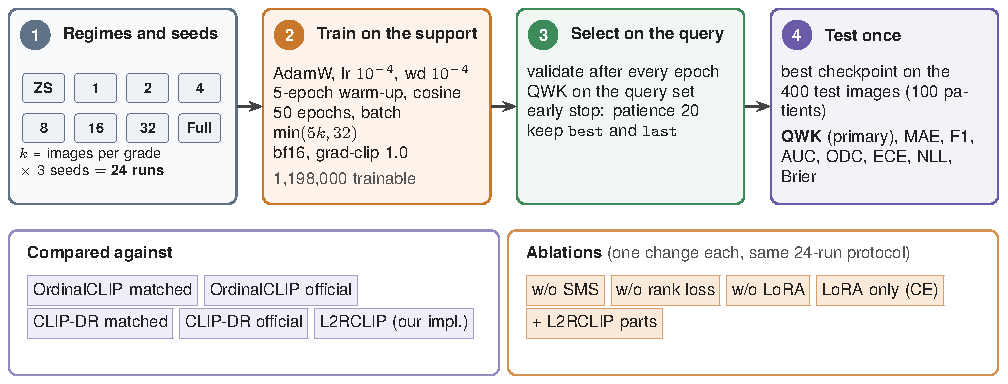
\includegraphics[width=\linewidth]{protocol_master}
\caption{\lr{protocol} آزمایش‌های مدل پایه: \lr{regime}ها و تکرارها، بهینه‌سازی، انتخاب مدل، اندازهٔ مدل، \lr{baseline}ها و \lr{ablation}ها.}
\label{fig:proto-master}
\end{figure}

\begin{figure}[H]
\begin{diagram}
  \node[train=2.6cm] (a1) {master: our model};
  \node[train=2.6cm,right=4mm of a1] (a2) {Dir.~1};
  \node[train=2.6cm,right=4mm of a2] (a3) {Dir.~2};
  \node[train=2.6cm,right=4mm of a3] (a4) {Dir.~3};
  \node[datan=5.4cm,below=14mm of $(a2)!0.5!(a3)$] (c) {Shared run cache\\ key = config hash};
  \node[box=5.4cm,below=of c] (q) {Compare main models\\ QWK · MAE · ODC · ECE · NLL};
  \node[decision,below=of q] (w) {Best branch};
  \node[train=5.4cm,below=of w] (p2) {Phase 2: baselines \& ablations of best branch};
  \node[lossn=5.4cm,below=of p2] (r) {Final report: tables, $k$-curves, confusion matrices};
  \foreach \a in {a1,a2,a3,a4} \draw[arr] (\a.south) -- (\a.south |- c.north);
  \draw[arr] (c)--(q); \draw[arr] (q)--(w); \draw[arr] (w)--(p2); \draw[arr] (p2)--(r);
  \draw[darr] (p2.west) -- ++(-12mm,0) |- (c.west);
  \begin{scope}[on background layer]\node[group,fit=(a1)(a4)] (g1) {};\end{scope}
  \node[grouplabel,anchor=south] at (g1.north) {Phase 1 · main models (24 runs each)};
\end{diagram}
\caption{گردش کار دو مرحله‌ای. اجرای تکراری یک \lr{configuration} در هیچ \lr{notebook}‌ای دوباره آموزش داده نمی‌شود.}
\label{fig:phases}
\end{figure}

\section{جهت ۱: هندسهٔ ترتیبی مستقیم}
\label{sec:d1}
\begin{keybox}[شاخه: \branch{direction1-ordinal-geometry}]
پنج \lr{grade vector} مستقیماً در فضای مشترک تصویر و متن آموخته می‌شوند و ترتیب، با سه \lr{constraint} هندسی \lr{ladder}، \lr{path} و \lr{anchor}، روی خود همین بردارها اعمال می‌شود. \lr{text encoder} فقط یک بار برای \lr{initialisation} به کار می‌رود.
\end{keybox}

شکل~\ref{fig:wf-d1} گردش کار کامل جهت ۱ را نشان می‌دهد. داده و تقسیم آن همان مدل پایه است و تفاوت در \lr{block}های مدل (الف) و \lr{loss function} (ب) است؛ \lr{protocol} آزمایش‌ها در شکل~\ref{fig:proto-d1} آمده است.

\begin{landscape}
\begin{figure}[p]
\centering
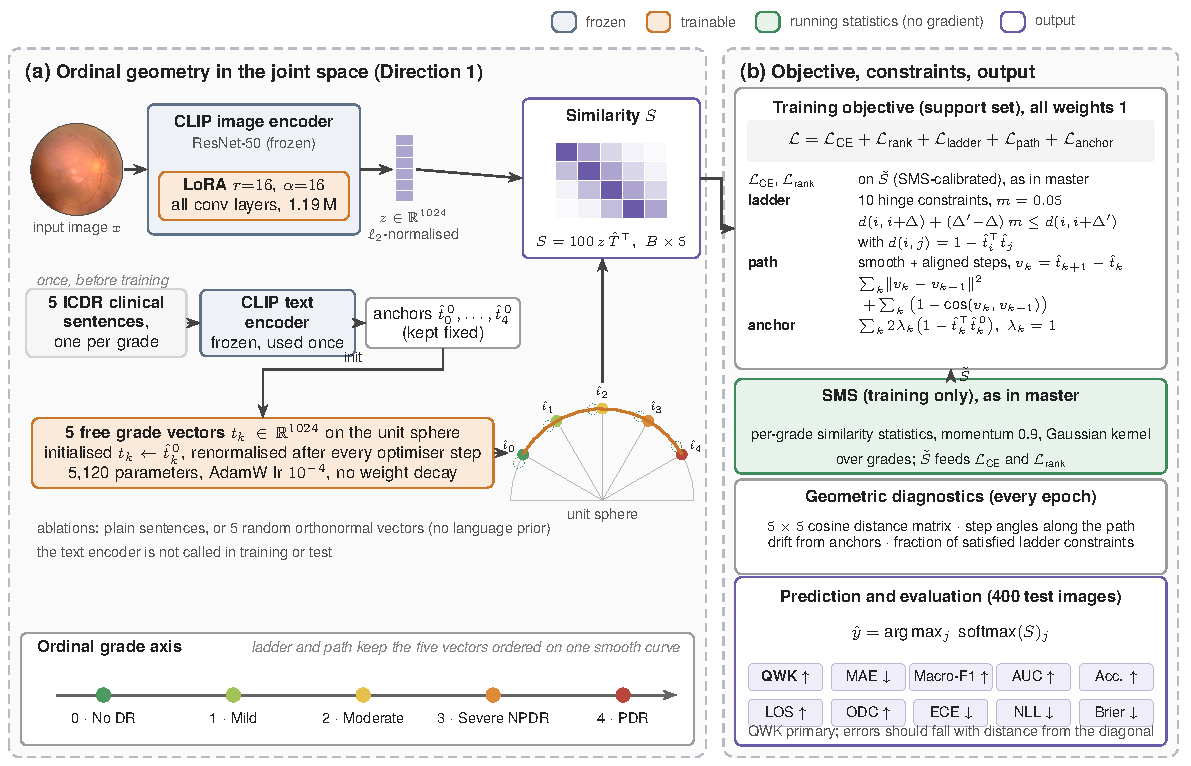
\includegraphics[width=\linewidth]{workflow_d1}
\caption{گردش کار کامل جهت ۱: بردارهای آزاد درجه که یک بار از جمله‌های بالینی مقداردهی می‌شوند، \lr{constraint}های \lr{ladder}، \lr{path} و \lr{anchor} روی همان بردارها و \lr{geometric diagnostics} هر \lr{epoch}.}
\label{fig:wf-d1}
\end{figure}
\end{landscape}

% ------------------------------------------------------------------
\subsection{انگیزه و شکاف پژوهشی}
در مدل پایه، ترتیب از راه توکن‌های ورودی \lr{text encoder} وارد می‌شود. \lr{rank token}ها شاید به هم نزدیک باشند، اما \lr{text encoder} یک تابع غیرخطی و \lr{frozen} است و هیچ تضمینی نیست که \lr{prototype}ها خروجی، یعنی همان بردارهایی که \lr{similarity} با آن‌ها سنجیده می‌شود، ترتیب را حفظ کنند. از سوی دیگر روش‌های جدید \lr{few-shot} مانند \lr{CLAP} \cite{clap} \lr{prototype}ها را مستقیماً در فضای مشترک می‌آموزند و با یک \lr{anchor} به متن اولیه نزدیک نگه می‌دارند؛ اما این روش‌ها هیچ رابطه‌ای میان کلاس‌ها در نظر نمی‌گیرند. جهت ۱ این دو را ترکیب می‌کند: پنج \lr{grade vector} مستقیماً در فضای مشترک آموخته می‌شوند و ترتیب، با \lr{geometric constraints}، روی خود همین بردارها اعمال می‌شود.

\begin{figure}[H]
\begin{diagram}
  \node[frozen=3.6cm] (a) {\textbf{Master model}\\ order injected into text encoder input};
  \node[box=3.6cm,below=of a] (a2) {Frozen nonlinear encoder may break ordering};
  \node[frozen=3.6cm,left=14mm of a] (b) {\textbf{CLAP}\\ free prototype + anchor};
  \node[box=3.6cm,below=of b] (b2) {No inter-class relationship is modelled};
  \node[train=6cm,below=12mm of $(a2)!0.5!(b2)$] (c) {\textbf{Dir.~1:} free grade vector + geometric ordinal constraints on those vectors};
  \draw[arr] (a)--(a2); \draw[arr] (b)--(b2); \draw[arr] (a2)--(c); \draw[arr] (b2)--(c);
\end{diagram}
\caption{شکاف پژوهشی جهت ۱: ترکیب \lr{prototype} آزاد (مانند \lr{CLAP}) با \lr{constraint} ترتیبی مستقیم.}
\label{fig:d1-gap}
\end{figure}

% ------------------------------------------------------------------
\subsection{تفاوت با مدل پایه}
\begin{table}[H]
\caption{آنچه در جهت ۱ تغییر می‌کند و آنچه ثابت می‌ماند}
\label{tab:d1-diff}
\centering\small
\begin{tabularx}{\textwidth}{@{}p{3.6cm} X X@{}}
\toprule
\textbf{جزء} & \textbf{مدل پایه} & \textbf{جهت ۱}\\
\midrule
نمایش درجه‌ها & \lr{prompt} \lr{learnable} از \lr{text encoder} \lr{frozen} & پنج بردار آزاد ۱۰۲۴-بعدی روی \lr{unit sphere}\\
\lr{text encoder} در آموزش & در هر گام فراخوانی می‌شود & فقط یک بار برای \lr{initialisation}\\
\lr{constraint} ترتیبی روی نمایش & \lr{interpolation} توکن‌ها & \lr{distance ladder}، \lr{smooth path}، \lr{anchor} به متن\\
\lr{image branch}، داده، \lr{SMS}، \lr{loss} رتبه، \lr{metric}ها، آموزش & \multicolumn{2}{l}{یکسان (بخش‌های \ref{sec:data} تا \ref{sec:metrics})}\\
\bottomrule
\end{tabularx}
\end{table}

% ------------------------------------------------------------------
\subsection{معماری}
\begin{figure}[H]
\begin{diagram}
  \node[datan=3.2cm] (s) {5 ICDR clinical sentences};
  \node[frozen=3.2cm,right=8mm of s] (te) {CLIP text encoder (frozen)};
  \node[datan=3.2cm,right=8mm of te] (t0) {$t^0_0\dots t^0_4$: anchors};
  \node[train=3.6cm,below=12mm of t0] (t) {$t_0\dots t_4$: free parameters\\ normalise after each step};
  \node[datan=2.6cm,left=46mm of t] (x) {Image};
  \node[train=3cm,below=of x] (v) {CLIP RN50 + LoRA};
  \node[box=3.6cm,below=of t] (g) {Geometric constraints:\\ ladder · path · anchor};
  \node[box=3.4cm,below=16mm of $(v)!0.5!(t)$] (sim) {$s = 100\cdot z\,\hat{t}^{\top}$};
  \node[box=3cm,below=of sim] (sms) {SMS (train only)};
  \node[lossn=3.4cm,below=of sms] (l1) {CE + rank-aware loss};
  \node[lossn=3.4cm,right=10mm of l1] (lg) {Geometric losses};
  \node[lossn=6cm,below=of $(l1)!0.5!(lg)$] (lt) {Total loss, Eq.~\ref{eq:d1-loss}};
  \draw[arr] (s)--(te); \draw[arr] (te)--(t0); \draw[arr] (t0)--node[elabel,right]{init}(t);
  \draw[arr] (x)--(v); \draw[arr] (v) |- (sim); \draw[arr] (t) -- (sim);
  \draw[arr] (sim)--(sms); \draw[arr] (sms)--(l1);
  \draw[arr] (t)--(g); \draw[darr] (t0.east) -- ++(5mm,0) |- (g.east);
  \draw[arr] (g) -- (lg); \draw[arr] (l1)--(lt); \draw[arr] (lg)--(lt);
  \begin{scope}[on background layer]\node[group,fit=(s)(te)(t0)] (gi) {};\end{scope}
  \node[grouplabel,anchor=south] at (gi.north) {Once, before training};
\end{diagram}
\archlegend
\caption{معماری جهت ۱. \lr{text encoder} فقط در \lr{initialisation} به کار می‌رود و در آموزش و آزمون حذف می‌شود.}
\label{fig:d1-arch}
\end{figure}

% ------------------------------------------------------------------
\subsection{\lr{initialisation} \lr{grade vector}ها}
هر \lr{grade vector} با کدگذاری یک جملهٔ بالینی مطابق مقیاس \lr{ICDR} \cite{icdr} توسط \lr{text encoder} \lr{frozen} آغاز می‌شود و نسخهٔ نرمال‌شدهٔ همین بردار به‌عنوان \lr{anchor} $\hat{t}^{0}_k$ نگه داشته می‌شود. در \lr{ablation}ها دو مقداردهی دیگر هم بررسی می‌شود: جمله‌های ساده (برای نمونه \lr{``A fundus photograph with mild non-proliferative diabetic retinopathy.''}) و پنج بردار متعامد تصادفی بدون هیچ دانش زبانی.

\begin{table}[H]
\caption{جمله‌های بالینی \lr{initialisation} (به زبان اصلی، همان‌گونه که به \lr{encoder} داده می‌شوند)}
\label{tab:d1-sent}
\centering\small
\begin{tabularx}{\textwidth}{@{}c X@{}}
\toprule
\textbf{درجه} & \textbf{جمله}\\
\midrule
۰ & \ensent{A fundus photograph showing no diabetic retinopathy, with normal retinal vasculature and no microaneurysms or hemorrhages.}\\
۱ & \ensent{A fundus photograph showing mild non-proliferative diabetic retinopathy, characterized by the presence of microaneurysms only.}\\
۲ & \ensent{A fundus photograph showing moderate non-proliferative diabetic retinopathy, with multiple microaneurysms, dot and blot hemorrhages, hard exudates, or cotton wool spots, less than severe.}\\
۳ & \ensent{A fundus photograph showing severe non-proliferative diabetic retinopathy, with extensive intraretinal hemorrhages in four quadrants, venous beading, or intraretinal microvascular abnormalities.}\\
۴ & \ensent{A fundus photograph showing proliferative diabetic retinopathy, characterized by neovascularization on the optic disc or elsewhere, vitreous hemorrhage, or preretinal hemorrhage.}\\
\bottomrule
\end{tabularx}
\end{table}

\begin{figure}[H]
\begin{diagram}
  \node[decision] (q) at (0,0) {Init type};
  \node[train=3.4cm] (a) at (-4.2,-2.0) {ICDR clinical sentences\\ (main model)};
  \node[box=3.4cm] (b) at (0,-2.0) {Plain sentences\\ (ablation)};
  \node[box=3.4cm] (c) at (4.2,-2.0) {5 random orthonormal\\ vectors (ablation)};
  \node[frozen=7.6cm] (e) at (-2.1,-3.75) {Frozen CLIP text encoder, then $\ell_2$-normalise};
  \node[datan=11.8cm] (o) at (0,-5.3) {$t_k \leftarrow \hat{t}^{\,0}_k$ \quad and keep $\hat{t}^{\,0}_k$ fixed as the anchor};
  \draw[arr] (q.west) -| (a.north);
  \draw[arr] (q.south) -- (b.north);
  \draw[arr] (q.east) -| (c.north);
  \draw[arr] (a.south) -- (a.south |- e.north);
  \draw[arr] (b.south) -- (b.south |- e.north);
  \draw[arr] (e.south) -- (e.south |- o.north);
  \draw[arr] (c.south) -- (c.south |- o.north);
  \node[elabel,right=1mm] at ($(c.south)!0.5!(c.south |- o.north)$) {no text encoder};
\end{diagram}
\caption{سه گزینهٔ مقداردهی \lr{grade vector}ها.}
\label{fig:d1-init}
\end{figure}

% ------------------------------------------------------------------
\subsection{\lr{ordinal geometric constraints}}
همهٔ \lr{constraint}ها روی بردارهای نرمال‌شدهٔ $\hat{t}_k$ و با \lr{cosine distance} $d(i, j) = 1 - \hat{t}_i^{\top} \hat{t}_j$ تعریف می‌شوند.

\subsubsection{\lr{distance ladder}}
از دید هر درجه، درجهٔ نزدیک‌تر باید از درجهٔ دورتر نزدیک‌تر باشد و این تفاوت با فاصلهٔ درجه‌ها \lr{margin}‌ای متناسب داشته باشد. برای پنج درجه، ۱۰ \lr{constraint} از این نوع وجود دارد:
\begin{equation}
\mathcal{L}_{\mathrm{ladder}} = \sum_{i} \sum_{1 \le \Delta < \Delta' \le K-1-i} \max\!\Big(0,\ d(i, i{+}\Delta) - d(i, i{+}\Delta') + (\Delta' - \Delta)\, m\Big), \qquad m = 0.05
\label{eq:ladder}
\end{equation}

\subsubsection{\lr{smooth path}}
پنج بردار باید روی یک خم یک‌بعدی و هموار روی \lr{sphere} قرار بگیرند تا ترتیب درجه‌ها در هندسه دیده شود. با گام‌های $v_k = \hat{t}_{k+1} - \hat{t}_k$، دو جزء تعریف می‌شود: هموار بودن (مشتق دوم کوچک) و هم‌جهت بودن گام‌های پیاپی:
\begin{equation}
\begin{gathered}
\mathcal{L}_{\mathrm{smooth}} = \sum_{k=1}^{K-2} \lVert v_k - v_{k-1} \rVert^2, \qquad \mathcal{L}_{\mathrm{align}} = \sum_{k=1}^{K-2} \big(1 - \cos(v_k, v_{k-1})\big),\\
\mathcal{L}_{\mathrm{path}} = \mathcal{L}_{\mathrm{smooth}} + \mathcal{L}_{\mathrm{align}}
\end{gathered}
\label{eq:path}
\end{equation}

\subsubsection{\lr{anchor}}
در \lr{regime} \lr{1-shot} یا \lr{2-shot}، بردارهای آزاد به‌آسانی \lr{overfitting} می‌کنند و دانش زبانی اولیه را از دست می‌دهند. \lr{anchor} هر بردار را به نقطهٔ آغازش نزدیک نگه می‌دارد. روی \lr{unit sphere}، مجذور \lr{Euclidean distance} برابر $2(1 - \cos)$ است:
\begin{equation}
\mathcal{L}_{\mathrm{anchor}} = \sum_k \lambda_k \lVert \hat{t}_k - \hat{t}^{0}_k \rVert^2 = \sum_k 2 \lambda_k \big(1 - \hat{t}_k^{\top} \hat{t}^{0}_k\big)
\label{eq:anchor}
\end{equation}
در مدل اصلی همهٔ $\lambda_k$ برابر ۱ هستند. دو وزن‌دهی دیگر در \lr{ablation} بررسی می‌شوند: وزن متناسب با معکوس ریشهٔ فراوانی هر درجه در دادهٔ آموزش (با میانگین ۱)، و وزن \lr{CLAP} که برابر میانگین احتمال \lr{zero-shot} درجهٔ درست روی تصاویر \lr{support} همان درجه است.

\begin{figure}[H]
\centering
\begin{latin}
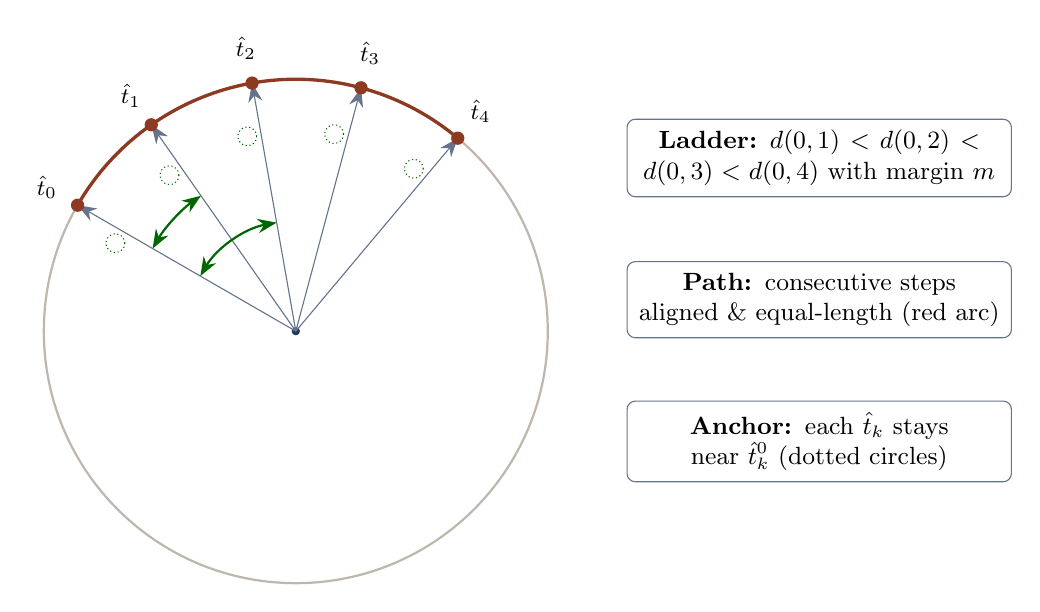
\begin{tikzpicture}[x=1cm,y=1cm]
  % sphere arc with five grade vectors
  \draw[rulegray,thick] (0,0) circle (3.2);
  \fill[navy] (0,0) circle (1.5pt);
  \foreach \a/\k/\n in {150/0/0,125/1/1,100/2/2,75/3/3,50/4/4} {
    \draw[->,navy!70] (0,0) -- (\a:3.2);
    \fill[accent] (\a:3.2) circle (2.4pt);
    \node[font=\footnotesize] at (\a:3.65) {$\hat t_{\k}$};
  }
  \draw[accent,very thick] (150:3.2) arc (150:50:3.2);
  \foreach \a in {154,129,104,79,54} \draw[densely dotted,green!40!black] (\a:2.55) circle (0.12);
  \draw[<->,thick,green!40!black] (150:2.1) arc (150:125:2.1);
  \draw[<->,thick,green!40!black] (150:1.4) arc (150:100:1.4);
  \node[box=4.6cm,anchor=west] at (4.2,2.2) {\textbf{Ladder:} $d(0,1)<d(0,2)<d(0,3)<d(0,4)$ with margin $m$};
  \node[box=4.6cm,anchor=west] at (4.2,0.4) {\textbf{Path:} consecutive steps aligned \& equal-length (red arc)};
  \node[box=4.6cm,anchor=west] at (4.2,-1.4) {\textbf{Anchor:} each $\hat t_k$ stays near $\hat t^0_k$ (dotted circles)};
\end{tikzpicture}
\end{latin}
\caption{سه \lr{constraint} هندسی روی \lr{grade vector}ها. \lr{ladder} ترتیب فاصله‌ها، مسیر شکل کلی و \lr{anchor} پیوند با دانش زبانی را حفظ می‌کند.}
\label{fig:d1-geom}
\end{figure}

% ------------------------------------------------------------------
\subsection{\lr{loss function} کل}
\begin{equation}
\mathcal{L} = \mathcal{L}_{\mathrm{CE}}(\tilde{s}, y) + \mathcal{L}_{\mathrm{rank}}(\tilde{s}, y) + \mathcal{L}_{\mathrm{ladder}} + \mathcal{L}_{\mathrm{path}} + \mathcal{L}_{\mathrm{anchor}}
\label{eq:d1-loss}
\end{equation}
همهٔ وزن‌ها برابر ۱ هستند و $\tilde{s}$ همان \lr{similarity} \lr{calibrated} با \lr{SMS} است (رابطهٔ~\ref{eq:sms}). \lr{distance-weighted pairwise loss} (رابطهٔ~\ref{eq:pair}) در مدل اصلی جهت ۱ وجود ندارد و فقط در \lr{ablation} «+ \lr{pairwise loss}» افزوده می‌شود.

\begin{table}[H]
\caption{اجزای \lr{loss function} جهت ۱}
\label{tab:d1-loss}
\centering\small
\begin{tabularx}{\textwidth}{@{}p{3cm} p{2.6cm} c X@{}}
\toprule
\textbf{جزء} & \textbf{روی چه چیزی} & \textbf{وزن} & \textbf{نقش}\\
\midrule
\lr{cross-entropy} & $\tilde{s}$ & ۱ & طبقه‌بندی درست\\
\lr{ranking-aware loss} & $\tilde{s}$ & ۱ & شکل \lr{unimodal} \lr{similarity} هر تصویر\\
\lr{ladder} (\ref{eq:ladder}) & $\hat t_k$ & ۱ & ترتیب فاصله‌ها میان درجه‌ها\\
مسیر (\ref{eq:path}) & $\hat t_k$ & ۱ & قرار گرفتن درجه‌ها روی یک خم هموار\\
\lr{anchor} (\ref{eq:anchor}) & $\hat t_k,\hat t^0_k$ & ۱ & جلوگیری از \lr{overfitting} و حفظ دانش زبانی\\
\bottomrule
\end{tabularx}
\end{table}

% ------------------------------------------------------------------
\subsection{بهینه‌سازی}
\lr{grade vector}ها با \lr{AdamW} و همان \lr{learning rate} $10^{-4}$ اما بدون \lr{weight decay} آموخته می‌شوند، چون \lr{weight decay} روی \lr{parameter}ی که دوباره به \lr{sphere} تصویر می‌شود فقط اندازهٔ گام مؤثر را تغییر می‌دهد. پس از هر گام \lr{optimizer}، هر بردار دوباره به طول واحد نرمال می‌شود. بقیهٔ تنظیمات همان جدول~\ref{tab:train} است. \lr{parameter}های \lr{trainable} \LRE{۱٬۱۸۸٬۲۷۲} (\lr{LoRA}) به‌اضافهٔ $5\times1024$ = \LRE{۵٬۱۲۰} (\lr{grade vector}ها)، در مجموع \LRE{۱٬۱۹۳٬۳۹۲} هستند.

\begin{figure}[H]
\begin{diagram}
  \node[box=3cm] (f) {Compute total loss};
  \node[box=3cm,right=of f] (b) {Backpropagation};
  \node[train=3.2cm,right=of b] (o) {AdamW step\\ LoRA: weight decay $10^{-4}$\\ $t$: no weight decay};
  \node[train=3cm,below=of o] (n) {$t_k \leftarrow t_k/\lVert t_k\rVert$};
  \node[box=3cm,left=of n] (d) {End of epoch: log geometric diagnostics};
  \draw[arr] (f)--(b); \draw[arr] (b)--(o); \draw[arr] (o)--(n); \draw[arr] (n)--(d); \draw[darr] (d) -| (f);
\end{diagram}
\caption{یک گام بهینه‌سازی در جهت ۱. \lr{normalisation} پس از هر گام بردارها را روی \lr{sphere} نگه می‌دارد.}
\label{fig:d1-opt}
\end{figure}

% ------------------------------------------------------------------
\subsection{داده، ارزیابی و \lr{geometric diagnostics}}
داده، \lr{protocol} \lr{few-shot}، \lr{preprocessing} و همهٔ \lr{metric}های بخش~\ref{sec:metrics} بدون تغییر به کار می‌روند: ۲۴ اجرا برای مدل اصلی ($k \in \{-1, 0, 1, 2, 4, 8, 16, 32\}$ با ۳ \lr{seed})، آزمون روی ۴۰۰ تصویر و \lr{QWK} به‌عنوان \lr{metric} اصلی. در حالت \lr{zero-shot}، مدل همان \lr{classifier} \lr{zero-shot} \lr{CLIP} با جمله‌های بالینی است. افزون بر \lr{metric}ها، در پایان هر \lr{epoch} چهار تشخیص هندسی ذخیره می‌شود:
\begin{enumerate}[label=\arabic*.]
\item ماتریس \lr{cosine distance} $5\times5$ بین درجه‌ها؛
\item زاویهٔ چرخش میان گام‌های پیاپی \lr{path}؛
\item فاصلهٔ هر بردار از \lr{anchor}‌اش؛
\item سهم \lr{constraint}های \lr{ladder} برقرار (از ۱۰ \lr{constraint}).
\end{enumerate}

% ------------------------------------------------------------------
\subsection{\lr{baseline}ها و \lr{ablation}ها}
مقایسه شامل مدل \lr{master}، همهٔ مدل‌های جدول~\ref{tab:baselines} و دو نسخه از \lr{CLAP} است. \lr{CLAP} \lr{matched} با جمله‌های ساده آغاز می‌شود، وزن \lr{anchor} \lr{CLAP} را به کار می‌برد، فقط \lr{loss} \lr{CE} و \lr{anchor} دارد و \lr{LoRA} تصویر را حفظ می‌کند. \lr{CLAP} \lr{official} یک \lr{linear probe} روی ویژگی‌های \lr{frozen} است: بدون \lr{LoRA}، با \lr{SGD} و نرخ \LRE{۰٫۱} به مدت ۳۰۰ \lr{epoch} و بدون \lr{early stopping}.

\begin{table}[H]
\caption{\lr{ablation}ها جهت ۱}
\label{tab:d1-abl}
\centering\small
\begin{tabularx}{\textwidth}{@{}p{4.6cm} X@{}}
\toprule
\textbf{آزمایش} & \textbf{تغییر نسبت به مدل اصلی}\\
\midrule
بدون \lr{ladder} / بدون \lr{path} / بدون \lr{anchor} & وزن همان \lr{constraint} صفر\\
بدون \lr{geometric constraints} & هر سه \lr{constraint} صفر\\
فقط \lr{CE} و هندسه & بدون \lr{loss} رتبه و \lr{SMS}\\
مقداردهی با جمله‌های ساده & جمله‌های کوتاه به‌جای جمله‌های بالینی\\
مقداردهی متعامد تصادفی & بدون هیچ دانش زبانی\\
\lr{anchor} با معکوس ریشهٔ فراوانی & $\lambda_k \propto 1/\sqrt{N_k}$\\
+ \lr{pairwise loss} & افزودن \lr{distance-weighted pairwise loss}\\
\bottomrule
\end{tabularx}
\end{table}

\begin{figure}[H]
\centering
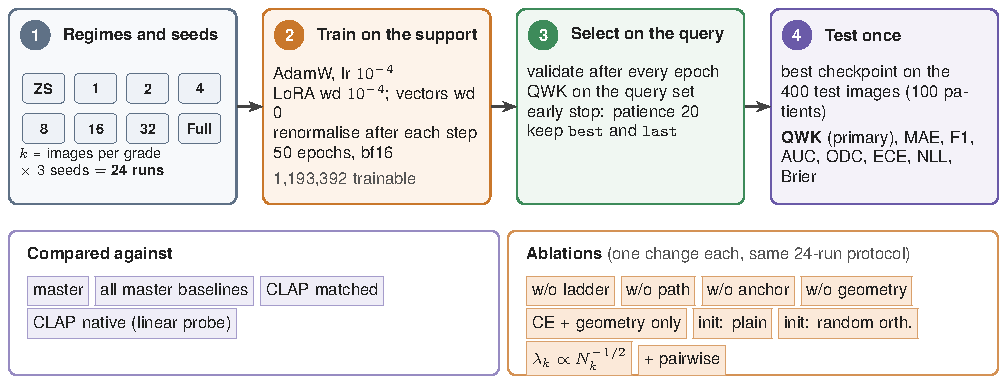
\includegraphics[width=\linewidth]{protocol_d1}
\caption{\lr{protocol} آزمایش‌های جهت ۱.}
\label{fig:proto-d1}
\end{figure}

\begin{figure}[H]
\begin{diagram}
  \node[train=4.4cm] (a) {Phase 1: Dir.~1 · 24 runs};
  \node[box=4.4cm,below=of a] (b) {Compare with master, Dir.~2 \& Dir.~3 from shared cache};
  \node[decision,below=of b] (c) {Dir.~1 is best?};
  \node[train=4.2cm,below=12mm of c,xshift=30mm] (d) {Phase 2: 9 baselines + 10 ablations};
  \node[box=4.2cm,below=12mm of c,xshift=-30mm] (e) {Tables from existing runs only};
  \node[lossn=4.2cm,below=of d] (f) {Geometric diagnostics for $k=8$};
  \draw[arr] (a)--(b); \draw[arr] (b)--(c);
  \draw[arr] (c) -| node[elabel,above,pos=0.3]{yes} (d); \draw[arr] (c) -| node[elabel,above,pos=0.3]{no} (e); \draw[arr] (d)--(f);
\end{diagram}
\caption{گردش کار آزمایش‌های جهت ۱.}
\label{fig:d1-flow}
\end{figure}

\section{جهت ۲: \lr{low-rank adaptation of the text encoder}}
\label{sec:d2}
\begin{keybox}[شاخه: \branch{direction2-ordinal-text-lora}]
درجه‌ها با ۲۵ توصیف بالینی واقعی بیان می‌شوند و خود \lr{text encoder} با \lr{LoRA} برای درجه‌بندی \lr{DR} تنظیم می‌شود. ترتیب روی خروجی \lr{text encoder} اعمال می‌شود، پس \lr{encoder} تطبیق‌یافته، و نه فقط پنج بردار، ترتیب درجه‌ها را می‌آموزد.
\end{keybox}

شکل~\ref{fig:wf-d2} گردش کار کامل جهت ۲ را نشان می‌دهد: ۲۵ توصیف بالینی از \lr{text encoder} تطبیق‌یافته با \lr{LoRA} می‌گذرند و \lr{constraint}های ترتیبی روی خروجی آن اعمال می‌شوند. \lr{protocol} آزمایش‌ها در شکل~\ref{fig:proto-d2} آمده است.

\begin{landscape}
\begin{figure}[p]
\centering
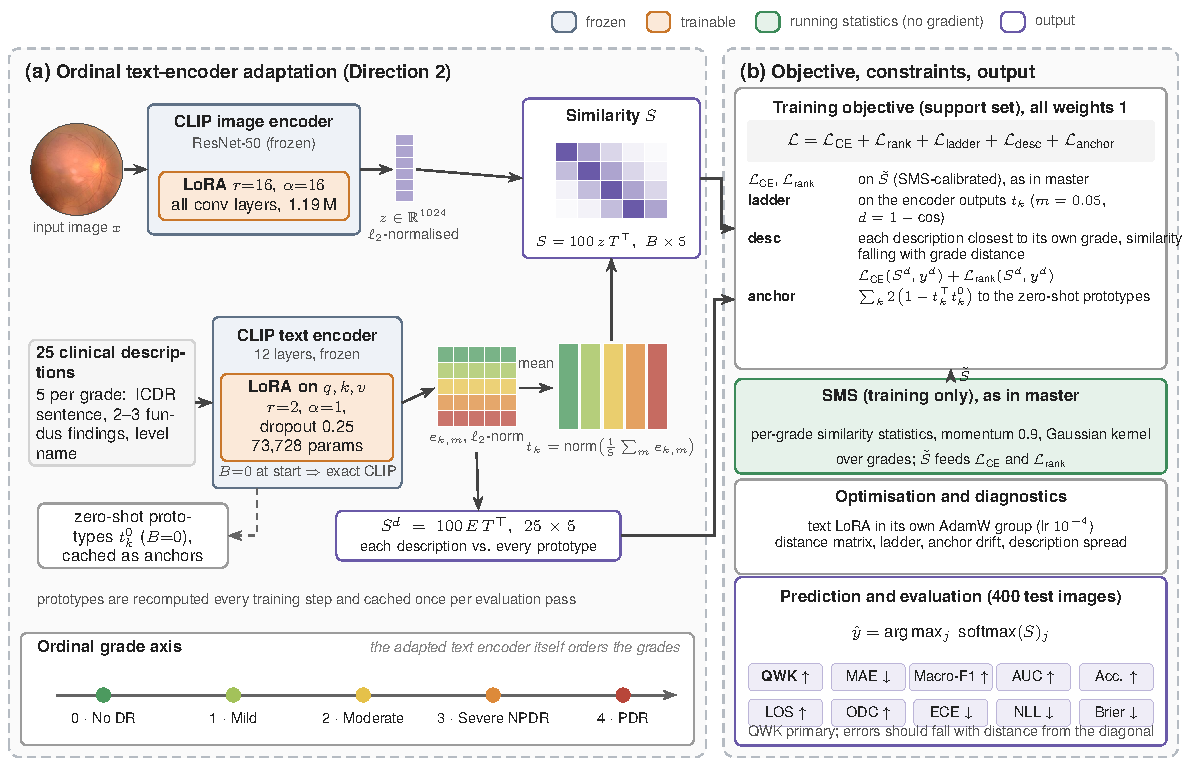
\includegraphics[width=\linewidth]{workflow_d2}
\caption{گردش کار کامل جهت ۲: توصیف‌های بالینی، \lr{LoRA} روی $q$، $k$ و $v$ \lr{text encoder}، \lr{prototype}ها میانگین، \lr{similarity matrix} توصیف‌ها $S^d$ و \lr{loss function} با \lr{constraint}های \lr{ladder}، \lr{description ordering} و \lr{anchor}.}
\label{fig:wf-d2}
\end{figure}
\end{landscape}

% ------------------------------------------------------------------
\subsection{انگیزه و شکاف پژوهشی}
مدل پایه \lr{prompt} را می‌آموزد و جهت ۱ \lr{grade vector}ها را؛ در هر دو، دانش زبانی فقط در نقطهٔ شروع حضور دارد. جهت ۲ برعکس عمل می‌کند: درجه‌ها با زبان بالینی واقعی توصیف می‌شوند و این بار خود \lr{text encoder}، با \lr{low-rank adaptation}، برای درجه‌بندی \lr{DR} تنظیم می‌شود. ایده از \lr{CLIP-LoRA} \cite{cliplora} گرفته شده که \lr{LoRA} را روی هر دو \lr{encoder} اعمال می‌کند، اما آن روش برای کلاس‌های بدون ترتیب طراحی شده است. نوآوری جهت ۲ این است که ترتیب روی خروجی \lr{text encoder} اعمال می‌شود. یک پیامد عملی هم دارد: توصیف تازه‌ای از یک درجه را می‌توان بدون آموزش دوباره کدگذاری کرد.

\begin{figure}[H]
\begin{diagram}
  \node[frozen=3.4cm] (a) {\textbf{Master / Dir.~1}\\ language knowledge only at init};
  \node[frozen=3.4cm,left=12mm of a] (b) {\textbf{CLIP-LoRA}\\ LoRA on both encoders, no ordering};
  \node[train=6.4cm,below=14mm of $(a)!0.5!(b)$] (c) {\textbf{Dir.~2:} clinical descriptions + text LoRA + ordinal constraint on text output};
  \node[datan=6.4cm,below=of c] (d) {Benefit: new description encoded without retraining};
  \draw[arr] (a) -- (c); \draw[arr] (b) -- (c); \draw[arr] (c)--(d);
\end{diagram}
\caption{شکاف پژوهشی جهت ۲.}
\label{fig:d2-gap}
\end{figure}

% ------------------------------------------------------------------
\subsection{تفاوت با مدل پایه}
\begin{table}[H]
\caption{آنچه در جهت ۲ تغییر می‌کند}
\label{tab:d2-diff}
\centering\small
\begin{tabularx}{\textwidth}{@{}p{3.6cm} X X@{}}
\toprule
\textbf{جزء} & \textbf{مدل پایه} & \textbf{جهت ۲}\\
\midrule
ورودی \lr{text branch} & توکن‌های \lr{learnable} & ۲۵ توصیف بالینی ثابت (۵ برای هر درجه)\\
\lr{text encoder} & \lr{frozen} & \lr{frozen} + \lr{LoRA} روی \lr{q}، \lr{k} و \lr{v} در هر ۱۲ لایه\\
\lr{prototype} درجه & خروجی یک \lr{prompt} & میانگین نرمال‌شدهٔ ۵ توصیف\\
\lr{constraint} ترتیبی روی نمایش & \lr{interpolation} توکن‌ها & \lr{ladder}، \lr{description ordering}، \lr{anchor}\\
\lr{image branch}، داده، \lr{SMS}، \lr{loss} رتبه، \lr{metric}ها، آموزش & \multicolumn{2}{l}{یکسان با بخش~\ref{sec:master}}\\
\bottomrule
\end{tabularx}
\end{table}

% ------------------------------------------------------------------
\subsection{معماری}
\begin{figure}[H]
\begin{diagram}
  \node[datan=3.6cm] (d) {25 clinical descriptions\\ 5 per grade};
  \node[train=3.6cm,below=of d] (te) {CLIP text encoder\\ frozen + LoRA on q, k, v};
  \node[box=3.6cm,below=of te] (e) {$e_{k,m}$: normalised description vector};
  \node[box=3.6cm,below=of e] (m) {Mean per grade + normalise: $t_0\dots t_4$};
  \node[datan=2.6cm,left=40mm of d] (x) {Image};
  \node[train=3cm,below=of x] (v) {CLIP RN50 + LoRA};
  \node[box=3.4cm,below=34mm of v] (s) {$s = 100\cdot z\,t^{\top}$};
  \node[box=2.6cm,below=of s] (sms) {SMS};
  \node[lossn=3.2cm,below=of sms] (l1) {CE + rank-aware loss};
  \node[lossn=2.4cm,below left=12mm and -14mm of m] (l2) {Ladder on $t$};
  \node[lossn=2.4cm,right=4mm of l2] (l4) {Anchor to zero-shot prototypes};
  \node[lossn=2.4cm,right=4mm of l4] (l3) {Desc.~ordering};
  \draw[arr] (d)--(te); \draw[arr] (te)--(e); \draw[arr] (e)--(m);
  \draw[arr] (x)--(v); \draw[arr] (v)--node[elabel,right]{$z$}(s); \draw[arr] (m) -- (s);
  \draw[arr] (s)--(sms); \draw[arr] (sms)--(l1);
  \draw[arr] (m)--(l2); \draw[arr] (m) -- (l4);
  \draw[arr] (e.east) -| (l3.north);
  \begin{scope}[on background layer]\node[group,fit=(d)(te)(e)(m)] (gt) {};\end{scope}
  \node[grouplabel,anchor=south] at (gt.north) {Text branch};
\end{diagram}
\archlegend
\caption{معماری جهت ۲. \lr{LoRA} متن و \lr{LoRA} تصویر هم‌زمان آموخته می‌شوند.}
\label{fig:d2-arch}
\end{figure}

% ------------------------------------------------------------------
\subsection{توصیف‌های بالینی}
برای هر درجه پنج توصیف به زبان انگلیسی نوشته شده است: جملهٔ بالینی جهت ۱، دو یا سه جمله دربارهٔ یافته‌های معمول فوندوس در آن درجه (میکروآنوریسم، خونریزی نقطه‌ای و لکه‌ای، اگزودای سخت، لکهٔ پنبه‌ای، تسبیحی شدن وریدها، ناهنجاری‌های ریزرگی درون شبکیه، نئوواسکولاریزاسیون) و یک جمله که سطح \lr{ICDR} را نام می‌برد. همهٔ توصیف‌ها در محدودهٔ ۷۷ توکن \lr{CLIP} جا می‌شوند. میانگین‌گیری چند توصیف (\lr{CuPL} \cite{cupl}) وابستگی \lr{prototype} به جمله‌بندی یک جملهٔ خاص را کم می‌کند.

\begin{table}[H]
\caption{نمونهٔ توصیف‌های درجهٔ ۳ (شدید غیرتکثیری)}
\label{tab:d2-desc}
\centering\small
\begin{tabularx}{\textwidth}{@{}c X@{}}
\toprule
\textbf{\#} & \textbf{توصیف}\\
\midrule
۱ & \ensent{A fundus photograph showing severe non-proliferative diabetic retinopathy, with extensive intraretinal hemorrhages in four quadrants, venous beading, or intraretinal microvascular abnormalities.}\\
۲ & \ensent{A retina with many intraretinal hemorrhages in all four quadrants and definite venous beading.}\\
۳ & \ensent{A color fundus image with intraretinal microvascular abnormalities and widespread hemorrhages but no new vessels.}\\
۴ & \ensent{Severe diabetic retinopathy meeting the 4-2-1 rule, without neovascularization.}\\
۵ & \ensent{Fundus photography graded as ICDR level 3, severe non-proliferative retinopathy.}\\
\bottomrule
\end{tabularx}
\end{table}

\begin{figure}[H]
\begin{diagram}
  \node[datan=3.6cm] (s1) {ICDR clinical sentence (Dir.~1)};
  \node[datan=3.6cm,right=4mm of s1] (s2) {2--3 fundus-finding sentences};
  \node[datan=3.6cm,right=4mm of s2] (s3) {ICDR level-name sentence};
  \node[box=6cm,below=12mm of s2] (e) {Encode each sentence and normalise: $e_{k,1}\dots e_{k,5}$};
  \node[train=6cm,below=of e] (t) {$t_k$ = normalised mean, Eq.~\ref{eq:d2-proto}};
  \draw[arr] (s1) |- (e.west); \draw[arr] (s2)--(e); \draw[arr] (s3) |- (e.east); \draw[arr] (e)--(t);
\end{diagram}
\caption{ساختن \lr{prototype} هر درجه از پنج توصیف.}
\label{fig:d2-desc}
\end{figure}

% ------------------------------------------------------------------
\subsection{\lr{low-rank adaptation of the text encoder}}
لایه‌های توجه \lr{text encoder} \lr{CLIP}، ماتریس‌های \lr{query}، کلید و مقدار را در یک ماتریس بسته‌بندی‌شده نگه می‌دارند و ابزارهای رایج \lr{LoRA} نمی‌توانند هر کدام را جداگانه هدف بگیرند. به همین دلیل، مطابق \lr{CLIP-LoRA}، هر \lr{attention block} با \lr{block}ی جایگزین می‌شود که وزن‌های \lr{frozen} را نگه می‌دارد و به‌روزرسانی کم‌رتبه را با \lr{dropout} روی ورودی می‌افزاید:
\begin{equation}
h_{\star} = W_{\star}\, x + \frac{\alpha}{r}\, B_{\star} A_{\star}\, \mathrm{dropout}(x), \qquad \star \in \{q, k, v\}
\label{eq:textlora}
\end{equation}
تنظیمات پیش‌فرض \lr{CLIP-LoRA} به کار می‌رود: $r=2$، $\alpha=1$ (ضریب \LRE{۰٫۵}) و \lr{dropout} \LRE{۰٫۲۵}، روی هر ۱۲ لایه. ماتریس $B$ با صفر آغاز می‌شود و آزمون نشان داده است که در این حالت خروجی \lr{encoder} دقیقاً با \lr{CLIP} اصلی برابر است. تعداد \lr{parameter}های \lr{LoRA} متن $12 \times 3 \times 2 \times 2 \times 512$ = \LRE{۷۳٬۷۲۸} است.
\begin{equation}
e_{k,m} = \frac{g_{\theta}(s_{k,m})}{\lVert g_{\theta}(s_{k,m}) \rVert}, \qquad t_k = \frac{\frac{1}{M} \sum_{m=1}^{M} e_{k,m}}{\big\lVert \frac{1}{M} \sum_{m} e_{k,m} \big\rVert}, \qquad M = 5
\label{eq:d2-proto}
\end{equation}
در ارزیابی، \lr{prototype}ها در طول یک دور ارزیابی تغییر نمی‌کنند و یک بار محاسبه می‌شوند. \lr{prototype}ها \lr{zero-shot} (با $B=0$) به‌عنوان \lr{anchor} $t^{0}_k$ نگه داشته می‌شوند.

\begin{figure}[H]
\begin{diagram}
  \node[datan=1.8cm] (x) {$x$ (tokens)};
  \node[frozen=3.6cm,right=12mm of x,yshift=12mm] (w) {$W_q,W_k,W_v$ frozen\\ (packed matrix)};
  \node[train=3.6cm,right=12mm of x,yshift=-12mm] (l) {dropout 0.25 $\rightarrow$ $A\ (r{=}2)$ $\rightarrow$ $B$ $\rightarrow$ $\times 0.5$};
  \node[circle,draw=navy,thick,inner sep=1pt,right=10mm of $(w.east)!0.5!(l.east)$] (p) {$+$};
  \node[frozen=2.8cm,right=8mm of p] (att) {Multi-head attention \& rest of layer};
  \draw[arr] (x) |- (w); \draw[arr] (x) |- (l); \draw[arr] (w) -| (p); \draw[arr] (l) -| (p); \draw[arr] (p)--(att);
\end{diagram}
\caption{\lr{attention block} بازنویسی‌شده با \lr{LoRA} روی \lr{q}، \lr{k} و \lr{v} (رابطهٔ~\ref{eq:textlora}).}
\label{fig:d2-lora}
\end{figure}

% ------------------------------------------------------------------
\subsection{\lr{constraint}های ترتیبی روی خروجی متن}
\paragraph{\lr{ladder} روی \lr{prototype}ها.} همان رابطهٔ~\ref{eq:ladder} جهت ۱، این بار روی $t_k$ که خروجی \lr{encoder} است.

\paragraph{\lr{description ordering}.} هر توصیف باید بیشترین \lr{similarity} را با درجهٔ خودش داشته باشد و \lr{similarity} آن با درجه‌های دیگر با فاصله کاهش یابد. \lr{similarity matrix} $25\times5$ توصیف‌ها و \lr{prototype}ها ساخته می‌شود و همان زوج \lr{loss} \lr{image branch} روی آن اعمال می‌شود:
\begin{equation}
S^{d}_{(k,m), j} = 100 \cdot e_{k,m}^{\top} t_j, \qquad \mathcal{L}_{\mathrm{desc}} = \mathcal{L}_{\mathrm{CE}}(S^{d}, y^{d}) + \mathcal{L}_{\mathrm{rank}}(S^{d}, y^{d})
\label{eq:desc}
\end{equation}
این \lr{constraint} ابر توصیف‌های هر درجه را از درجه‌های دیگر جدا و در امتداد محور درجه مرتب نگه می‌دارد. اگر \lr{encoder} برای کم کردن \lr{loss} تصویر، توصیف‌های دو درجهٔ همسایه را روی هم بیندازد، این \lr{constraint} جلوی آن را می‌گیرد.

\paragraph{\lr{anchor}.} رابطهٔ~\ref{eq:anchor} با $t^{0}_k$ \lr{zero-shot}، تا \lr{encoder} در \lr{regime} بسیار \lr{few-shot} از دانش اولیه دور نشود.

\begin{equation}
\mathcal{L} = \mathcal{L}_{\mathrm{CE}}(\tilde{s}, y) + \mathcal{L}_{\mathrm{rank}}(\tilde{s}, y) + \mathcal{L}_{\mathrm{ladder}} + \mathcal{L}_{\mathrm{desc}} + \mathcal{L}_{\mathrm{anchor}}
\label{eq:d2-loss}
\end{equation}
همهٔ وزن‌ها ۱ هستند. \lr{constraint} \lr{path} و \lr{pairwise loss} در مدل اصلی خاموش‌اند.

\begin{figure}[H]
\centering
\begin{latin}
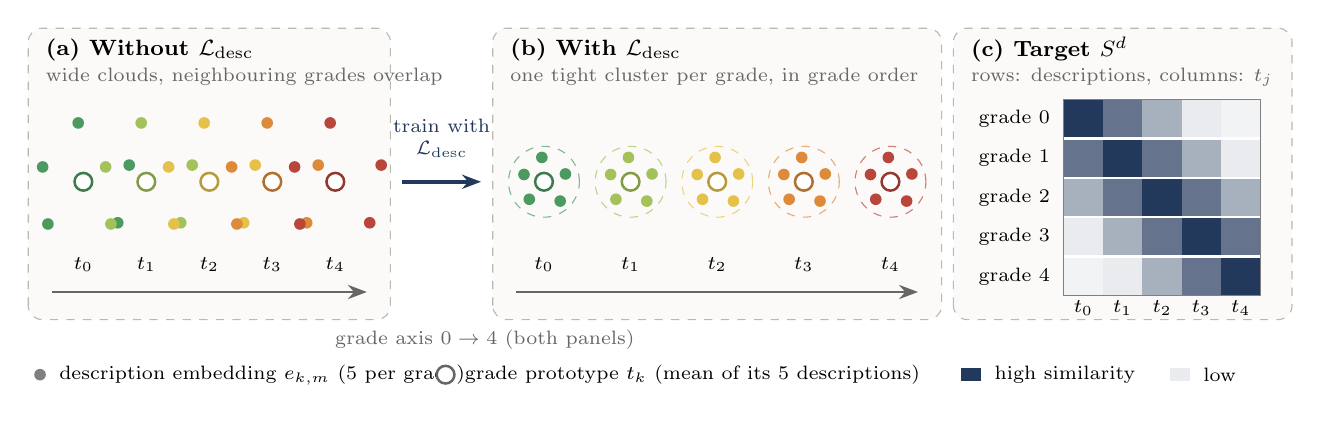
\begin{tikzpicture}[x=1cm,y=1cm,font=\footnotesize]
  \definecolor{q0}{HTML}{4C9A5F}\definecolor{q1}{HTML}{A3C25A}\definecolor{q2}{HTML}{E5C14A}
  \definecolor{q3}{HTML}{DD8A3A}\definecolor{q4}{HTML}{B8463A}
  \tikzset{pnl/.style={rulegray,dashed,rounded corners=5pt,fill=panel!40},
           ttl/.style={font=\footnotesize\bfseries,anchor=west},
           sub/.style={font=\scriptsize,text=black!60,anchor=west},
           proto/.style={line width=0.9pt,fill=white}}
  % common panel geometry: y from -1.75 to 1.95, title at 1.68, subtitle at 1.33, content centred at y=0
  % ---------- (a) without L_desc: same layout as (b) but wide, overlapping clouds ----------
  \draw[pnl] (0,-1.75) rectangle (4.6,1.95);
  \node[ttl] at (0.1,1.68) {(a) Without $\mathcal{L}_{\mathrm{desc}}$};
  \node[sub] at (0.1,1.33) {wide clouds, neighbouring grades overlap};
  \foreach \k/\c in {0/q0,1/q1,2/q2,3/q3,4/q4} {
    \foreach \a/\r in {20/0.62,95/0.75,160/0.55,230/0.7,310/0.68}
      \fill[\c] ($({0.7+0.8*\k},0)+(\a:\r)$) circle (2.1pt);}
  \foreach \k/\c in {0/q0,1/q1,2/q2,3/q3,4/q4} {
    \draw[\c!80!black,proto] ({0.7+0.8*\k},0) circle (3.2pt);
    \node[font=\scriptsize] at ({0.7+0.8*\k},-1.05) {$t_{\k}$};}
  \draw[->,line width=0.9pt,black!60] (0.3,-1.4) -- (4.3,-1.4);
  % ---------- arrow ----------
  \draw[->,line width=1.4pt,navy] (4.75,0) -- (5.75,0);
  \node[font=\scriptsize,align=center,text=navy] at (5.25,0.55) {train with\\ $\mathcal{L}_{\mathrm{desc}}$};
  % ---------- (b) with L_desc ----------
  \draw[pnl] (5.9,-1.75) rectangle (11.6,1.95);
  \node[ttl] at (6.0,1.68) {(b) With $\mathcal{L}_{\mathrm{desc}}$};
  \node[sub] at (6.0,1.33) {one tight cluster per grade, in grade order};
  \foreach \k/\c in {0/q0,1/q1,2/q2,3/q3,4/q4} {
    \draw[\c!70,dashed] ({6.55+1.1*\k},0) circle (0.45);
    \foreach \a/\r in {20/0.29,95/0.31,160/0.27,230/0.29,310/0.32} \fill[\c] ($({6.55+1.1*\k},0)+(\a:\r)$) circle (2.1pt);
    \draw[\c!80!black,proto] ({6.55+1.1*\k},0) circle (3.2pt);
    \node[font=\scriptsize] at ({6.55+1.1*\k},-1.05) {$t_{\k}$};}
  \draw[->,line width=0.9pt,black!60] (6.2,-1.4) -- (11.3,-1.4);
  % ---------- (c) target S^d ----------
  \draw[pnl] (11.75,-1.75) rectangle (16.05,1.95);
  \node[ttl] at (11.85,1.68) {(c) Target $S^{d}$};
  \node[sub] at (11.85,1.33) {rows: descriptions, columns: $t_j$};
  \foreach \k in {0,...,4} {
    \foreach \m in {0,...,4} {
      \foreach \j in {0,...,4} {
        \pgfmathtruncatemacro{\v}{max(6,100-30*abs(\k-\j))}
        \fill[navy!\v] ({13.15+0.5*\j},{1.05-0.1*(5*\k+\m)}) rectangle ++(0.5,-0.1);}}
    \draw[white,line width=0.8pt] (13.15,{1.05-0.5*\k}) -- (15.65,{1.05-0.5*\k});
    \node[anchor=east,font=\scriptsize] at (13.1,{0.8-0.5*\k}) {grade \k};}
  \draw[black!50] (13.15,1.05) rectangle (15.65,-1.45);
  \foreach \j in {0,...,4} \node[font=\scriptsize] at ({13.4+0.5*\j},-1.6) {$t_{\j}$};
  % shared axis label and legend under the panels
  \node[font=\scriptsize,text=black!60] at (5.8,-2.0) {grade axis $0\rightarrow4$ (both panels)};
  \fill[black!50] (0.15,-2.45) circle (2.1pt); \node[anchor=west,font=\scriptsize] at (0.27,-2.45) {description embedding $e_{k,m}$ (5 per grade)};
  \draw[black!60,proto] (5.3,-2.45) circle (3.2pt); \node[anchor=west,font=\scriptsize] at (5.42,-2.45) {grade prototype $t_k$ (mean of its 5 descriptions)};
  \fill[navy] (11.85,-2.53) rectangle ++(0.25,0.16); \node[anchor=west,font=\scriptsize] at (12.15,-2.45) {high similarity};
  \fill[navy!10] (14.5,-2.53) rectangle ++(0.25,0.16); \node[anchor=west,font=\scriptsize] at (14.8,-2.45) {low};
\end{tikzpicture}
\end{latin}
\caption{هدف \lr{description ordering} (رابطهٔ~\ref{eq:desc}). (الف) بدون این \lr{constraint}، توصیف‌های درجه‌های همسایه روی هم می‌افتند. (ب) \lr{cross-entropy} روی $S^d$ توصیف‌های هر درجه را دور \lr{prototype} همان درجه جمع می‌کند و \lr{ranking-aware loss} روی $S^d$ این خوشه‌ها را در امتداد محور درجه مرتب نگه می‌دارد. (ج) الگوی هدف ماتریس $S^d$: بیشترین \lr{similarity} هر توصیف با درجهٔ خودش است و با فاصلهٔ درجه کاهش می‌یابد.}
\label{fig:d2-clouds}
\end{figure}

% ------------------------------------------------------------------
\subsection{آموزش، داده و ارزیابی}
\lr{parameter}های \lr{LoRA} متن در یک گروه جداگانهٔ \lr{optimizer} با همان \lr{learning rate} $10^{-4}$ و \lr{weight decay} آموخته می‌شوند. بقیهٔ تنظیمات، داده، \lr{protocol} ۲۴ اجرایی و \lr{metric}ها همان بخش~\ref{sec:master} است و کل \lr{parameter}های \lr{trainable} \LRE{۱٬۱۸۸٬۲۷۲} + \LRE{۷۳٬۷۲۸} = \LRE{۱٬۲۶۲٬۰۰۰} است. در حالت \lr{zero-shot}، مدل همان \lr{classifier} \lr{zero-shot} \lr{CLIP} با میانگین ۲۵ توصیف است. تشخیص‌های هر \lr{epoch} علاوه بر موارد جهت ۱، پراکندگی توصیف‌های هر درجه گرد \lr{prototype}‌اش (میانگین $1-\cos$) را هم ثبت می‌کند.

% ------------------------------------------------------------------
\subsection{\lr{baseline}ها و \lr{ablation}ها}
دو مقایسهٔ اختصاصی این جهت عبارت‌اند از \lr{CLIP-LoRA} (\lr{LoRA} روی هر دو \lr{encoder}، \lr{prompt} قالبی \lr{``a photo of a \{grade\}.''} و فقط \lr{loss} \lr{CE}) و \lr{CLIP-LoRA} با \lr{loss}های ترتیبی ما (\lr{CE}، \lr{ranking-aware loss} و \lr{SMS}). مقایسهٔ دوم پاسخ می‌دهد که آیا \lr{constraint}های ترتیبی روی خروجی متن لازم‌اند یا \lr{loss}های سمت تصویر کافی است. مدل \lr{master}، جهت ۱ و مدل‌های جدول~\ref{tab:baselines} هم در مقایسه حضور دارند.

\begin{table}[H]
\caption{\lr{ablation}ها جهت ۲}
\label{tab:d2-abl}
\centering\small
\begin{tabularx}{\textwidth}{@{}p{5.2cm} X@{}}
\toprule
\textbf{آزمایش} & \textbf{تغییر نسبت به مدل اصلی}\\
\midrule
بدون \lr{ladder} / بدون \lr{description ordering} / بدون \lr{anchor} & وزن همان \lr{constraint} صفر\\
بدون \lr{constraint}های متنی & هر سه \lr{constraint} صفر\\
\lr{text encoder} \lr{frozen} & بدون \lr{LoRA} متن؛ \lr{prototype}ها ثابت و برابر میانگین \lr{zero-shot}\\
یک جملهٔ بالینی & فقط جملهٔ اول هر درجه\\
جمله‌های ساده & یک جملهٔ کوتاه برای هر درجه\\
رتبهٔ ۸ & $r=8,\ \alpha=4$\\
\lr{LoRA} روی \lr{q}، \lr{k}، \lr{v} و \lr{o} & افزودن تصویر خروجی توجه\\
+ \lr{pairwise loss} & افزودن \lr{distance-weighted pairwise loss}\\
\bottomrule
\end{tabularx}
\end{table}

\begin{figure}[H]
\centering
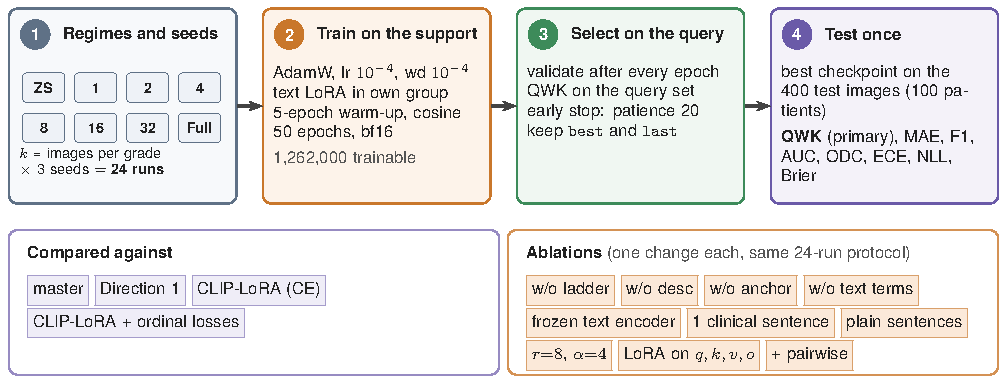
\includegraphics[width=\linewidth]{protocol_d2}
\caption{\lr{protocol} آزمایش‌های جهت ۲.}
\label{fig:proto-d2}
\end{figure}

\begin{figure}[H]
\begin{diagram}
  \node[train=4.4cm] (a) {Phase 1: Dir.~2 · 24 runs};
  \node[box=4.4cm,below=of a] (b) {Compare with master, Dir.~1 \& Dir.~3};
  \node[decision,below=of b] (c) {Dir.~2 is best?};
  \node[train=5cm,below=of c] (d) {Phase 2: CLIP-LoRA \& ordinal variant + 11 ablations};
  \node[lossn=5cm,below=of d] (e) {Diagnostics: ladder, desc.~spread, anchor distance};
  \draw[arr] (a)--(b); \draw[arr] (b)--(c); \draw[arr] (c)--node[elabel,right]{yes}(d); \draw[arr] (d)--(e);
\end{diagram}
\caption{گردش کار آزمایش‌های جهت ۲.}
\label{fig:d2-flow}
\end{figure}

\section{جهت ۳: نمایش احتمالاتی درجه‌ها}
\label{sec:d3}
\begin{keybox}[شاخه: \branch{direction3-probabilistic-ordinal}]
هر درجه یک \lr{von Mises--Fisher distribution} روی \lr{unit sphere} است: یک \lr{mean direction} که درجه را مکان‌یابی می‌کند و یک \lr{concentration} \lr{trainable} که ابهام آن درجه را نشان می‌دهد. \lr{mixture posterior} این توزیع‌ها جای \lr{softmax} \lr{similarity} را می‌گیرد و هدف دوم، \lr{calibration} احتمال‌هاست.
\end{keybox}

شکل~\ref{fig:wf-d3} گردش کار کامل جهت ۳ را نشان می‌دهد: هر درجه یک \lr{von Mises--Fisher distribution} با \lr{mean direction} و \lr{concentration} \lr{trainable} است و \lr{mixture posterior} آن‌ها جای \lr{softmax} \lr{similarity} را می‌گیرد. \lr{protocol} آزمایش‌ها در شکل~\ref{fig:proto-d3} آمده است.

\begin{landscape}
\begin{figure}[p]
\centering
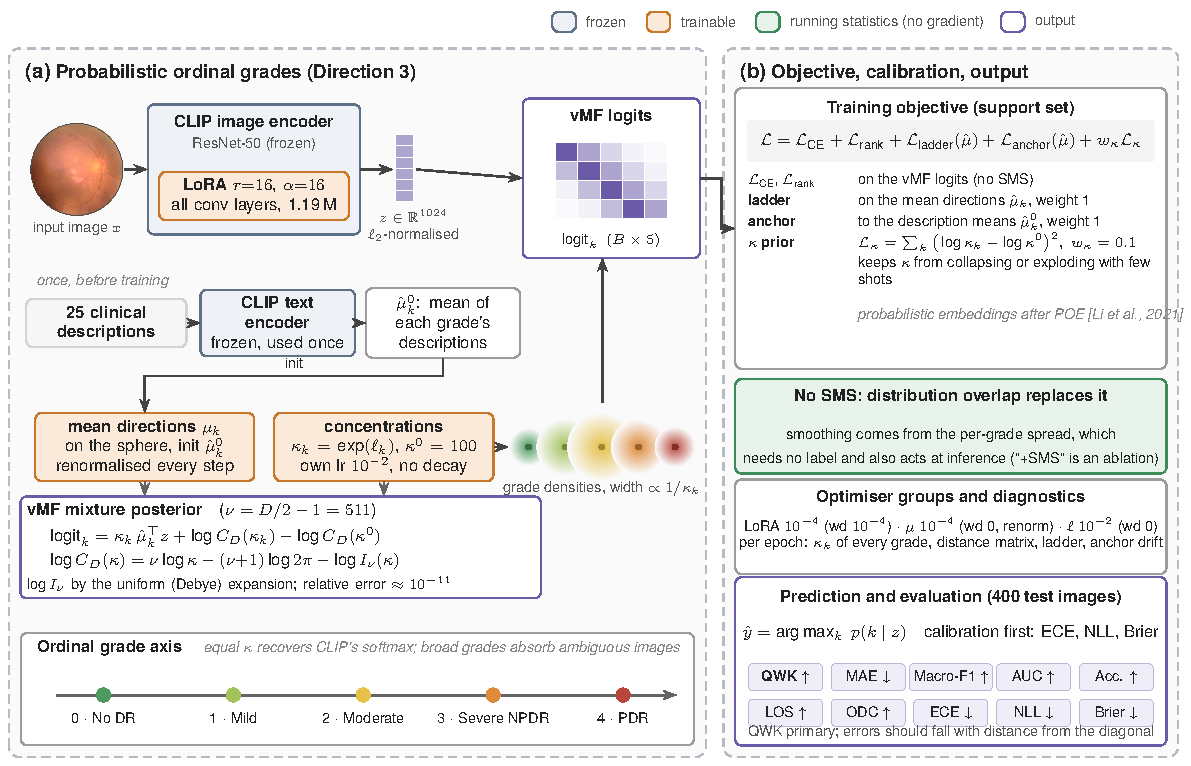
\includegraphics[width=\linewidth]{workflow_d3}
\caption{گردش کار کامل جهت ۳: \lr{mean direction}ها و \lr{concentration}های \lr{trainable}، \lr{mixture posterior} \lr{vMF} با محاسبهٔ پایدار \lr{Bessel function}، \lr{loss function} با \lr{concentration prior} و تأکید بر \lr{metric}های \lr{calibration}.}
\label{fig:wf-d3}
\end{figure}
\end{landscape}

% ------------------------------------------------------------------
\subsection{انگیزه و شکاف پژوهشی}
مرز درجه‌های \lr{DR} قطعی نیست و اختلاف نظر درجه‌بندها بیشتر میان درجه‌های ۱ و ۲ و میان ۲ و ۳ دیده می‌شود. یک \lr{prototype} تک‌نقطه‌ای نمی‌تواند این ابهام را نشان دهد. در جهت ۳ هر درجه یک توزیع روی \lr{unit sphere} است: یک \lr{mean direction} که درجه را مکان‌یابی می‌کند و یک \lr{concentration} که نشان می‌دهد درجه چقدر روشن تعریف شده است. نمایش احتمالاتی پیش‌تر در سمت تصویر بررسی شده است (\lr{POE} \cite{poe})، اما \lr{prototype}ها احتمالاتی سمت متن با \lr{constraint} ترتیبی، برای درجه‌بندی \lr{few-shot}، در مرور منابع این پژوهش یافت نشد. هدف دوم این جهت \lr{calibration} است: احتمال‌هایی که با دقت واقعی هم‌خوانی دارند، برای کاربرد بالینی ارزشمندند.

\begin{figure}[H]
\centering
\begin{latin}
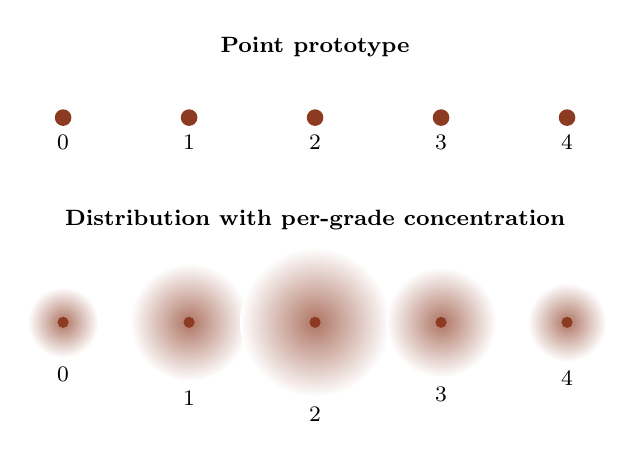
\begin{tikzpicture}[x=-1cm,y=1cm]
  \begin{scope}
    \foreach \x/\n in {0/0,-1.6/1,-3.2/2,-4.8/3,-6.4/4} {\fill[accent] (\x,0) circle (3pt); \node[below=3pt,font=\footnotesize] at (\x,0) {\n};}
    \node[font=\footnotesize\bfseries] at (-3.2,0.9) {Point prototype};
  \end{scope}
  \begin{scope}[yshift=-2.6cm]
    \foreach \x/\w/\n in {0/0.45/0,-1.6/0.75/1,-3.2/0.95/2,-4.8/0.7/3,-6.4/0.5/4} {
      \shade[inner color=accent!70,outer color=white] (\x,0) circle (\w);
      \fill[accent] (\x,0) circle (2pt); \node[below=\w cm,font=\footnotesize] at (\x,0) {\n};}
    \node[font=\footnotesize\bfseries] at (-3.2,1.3) {Distribution with per-grade concentration};
  \end{scope}
\end{tikzpicture}
\end{latin}
\caption{از نقطه به توزیع: درجه‌های مبهم‌تر (مانند ۱ تا ۳) می‌توانند \lr{concentration} کمتر و پراکندگی بیشتری بیاموزند.}
\label{fig:d3-idea}
\end{figure}

% ------------------------------------------------------------------
\subsection{مدل \lr{von Mises--Fisher} برای هر درجه}
\lr{von Mises--Fisher distribution} (\lr{vMF}) روی \lr{sphere} $S^{D-1}$ با \lr{mean direction} $\mu$ و \lr{concentration} $\kappa$ چنین است:
\begin{equation}
\mathrm{vMF}(z;\, \mu, \kappa) = C_D(\kappa)\, \exp(\kappa\, \mu^{\top} z), \qquad C_D(\kappa) = \frac{\kappa^{\nu}}{(2\pi)^{\nu+1} I_{\nu}(\kappa)}, \qquad \nu = \frac{D}{2} - 1 = 511
\label{eq:vmf}
\end{equation}
تابع $I_\nu$ \lr{modified Bessel function of the first kind} است. برای هر درجه، $\mu_k$ مانند جهت ۱ یک بردار آزاد روی \lr{sphere} است که از میانگین ۲۵ توصیف بالینی جهت ۲ (با \lr{encoder} \lr{frozen}) آغاز می‌شود، و $\kappa_k = \exp(\ell_k)$ با مقدار اولیهٔ ۱۰۰ آموخته می‌شود. این مقدار اولیه همان \lr{logit scale} \lr{CLIP} است.

% ------------------------------------------------------------------
\subsection{امتیازدهی: \lr{mixture posterior} \lr{vMF}}
تصویر با \lr{mixture posterior}‌ای از پنج توزیع طبقه‌بندی می‌شود. ثابت $\log C_D(\kappa^{0})$ برای همهٔ درجه‌ها یکسان است و در \lr{softmax} حذف می‌شود؛ کم کردن آن در \lr{double precision}، \lr{logit}ها را در مقیاس \lr{CLIP} نگه می‌دارد. مقدار $\log C_D$ در $\kappa=100$ حدود ۲۰۰۰+ است و جمع آن در \lr{single precision} حدود چهار رقم اعشار را از بین می‌برد:
\begin{equation}
\mathrm{logit}_k = \kappa_k\, \hat{\mu}_k^{\top} z + \log C_D(\kappa_k) - \log C_D(\kappa^{0}), \qquad p(k \mid z) = \operatorname{softmax}_k(\mathrm{logit}_k)
\label{eq:vmf-logit}
\end{equation}
دو ویژگی این امتیازدهی مهم است:
\begin{enumerate}[label=\arabic*.]
\item اگر همهٔ $\kappa_k$ برابر باشند، \lr{posterior} دقیقاً \lr{softmax} \lr{similarity} \lr{CLIP} با مقیاس $\kappa$ است؛ پس حالت \lr{zero-shot} همان \lr{classifier} \lr{zero-shot} با میانگین توصیف‌هاست.
\item اگر درجه‌ای پهن‌تر شود ($\kappa$ کمتر)، برای تصاویری که از همهٔ میانگین‌ها دورند احتمال بیشتری می‌گیرد؛ این همان رفتار هموارسازی است که \lr{SMS} به \lr{similarity}ها تحمیل می‌کند، اما اینجا جزء خود مدل است و در آزمون هم وجود دارد.
\end{enumerate}
در \lr{ablation}، امتیازدهی دیگری هم بررسی می‌شود: \lr{similarity} مورد انتظار با \lr{prototype}‌ای که از توزیع درجه برداشته شود. نسبت $A_D(\kappa) = I_{\nu+1}(\kappa) / I_{\nu}(\kappa)$ \lr{mean resultant length} است؛ برای نمونه $A_D(100) \approx 0.0967$ که با مقیاس \lr{similarity}های واقعی \lr{CLIP} هم‌خوانی دارد:
\begin{equation}
\mathrm{logit}_k = 100 \cdot \frac{A_D(\kappa_k)}{A_D(\kappa^{0})}\, \hat{\mu}_k^{\top} z
\label{eq:expected}
\end{equation}

% ------------------------------------------------------------------
\subsection{محاسبهٔ پایدار \lr{Bessel function}}
در مرتبهٔ $\nu=511$ تابع $I_\nu$ در دقت معمولی فرومی‌ریزد؛ برای نمونه، تابع \code{scipy.special.iv} در $\kappa=50$ مقدار صفر و در $\kappa=100$ مقداری از مرتبهٔ $10^{-294}$ برمی‌گرداند. به همین دلیل لگاریتم آن با \lr{uniform asymptotic expansion} (\lr{Debye expansion}) و نخستین جملهٔ تصحیحی محاسبه می‌شود \cite{dlmf}:
\begin{equation}
\begin{aligned}
\log I_{\nu}(\kappa) &\approx \eta - \tfrac{1}{2}\log(2\pi) - \tfrac{1}{4}\log(\nu^2 + \kappa^2) + \log\!\Big(1 + \frac{u_1(t)}{\nu}\Big),\\
\eta &= \sqrt{\nu^2 + \kappa^2} + \nu \log \frac{\kappa}{\nu + \sqrt{\nu^2 + \kappa^2}}, \qquad t = \frac{\nu}{\sqrt{\nu^2 + \kappa^2}}, \qquad u_1(t) = \frac{3t - 5t^3}{24}
\end{aligned}
\label{eq:bessel}
\end{equation}
این تقریب در بازهٔ $\kappa \in [1, 1000]$ با محاسبهٔ دقت دلخواه کتابخانهٔ \lr{mpmath} مقایسه شده و \lr{relative error} آن حدود $10^{-11}$ است. تقریب نسبت به $\kappa$ هموار و مشتق‌پذیر است و \lr{gradient} مستقیماً از آن عبور می‌کند.

\begin{figure}[H]
\begin{diagram}
  \node[train=2.4cm] (k) {$\ell_k$};
  \node[box=2.4cm,right=of k] (e) {$\kappa_k=e^{\ell_k}$};
  \node[box=3.6cm,right=of e] (b) {$\log I_\nu(\kappa_k)$\\ Debye expansion, Eq.~\ref{eq:bessel}};
  \node[box=3cm,below=of b] (c) {$\log C_D(\kappa_k)$\\ Eq.~\ref{eq:vmf}};
  \node[box=3cm,left=of c] (c0) {Subtract $\log C_D(\kappa^0)$ in float64};
  \node[lossn=3.2cm,left=of c0] (lg) {Logit, Eq.~\ref{eq:vmf-logit}};
  \draw[arr] (k)--(e); \draw[arr] (e)--(b); \draw[arr] (b)--(c); \draw[arr] (c)--(c0); \draw[arr] (c0)--(lg);
\end{diagram}
\caption{مسیر محاسبهٔ \lr{logit} \lr{vMF}. \lr{gradient} از همهٔ مراحل تا $\ell_k$ عبور می‌کند.}
\label{fig:d3-bessel}
\end{figure}

% ------------------------------------------------------------------
\subsection{معماری}
\begin{figure}[H]
\begin{diagram}
  \node[datan=3cm] (d) {25 clinical descriptions};
  \node[frozen=3cm,right=7mm of d] (te) {Frozen text encoder};
  \node[datan=3cm,right=7mm of te] (m0) {$\mu^0_k$: mean of descriptions per grade};
  \node[train=3.4cm,below=12mm of m0] (mu) {$\mu_k$: mean direction, free on sphere};
  \node[train=3.4cm,left=6mm of mu] (ka) {$\kappa_k=\exp(\ell_k)$: concentration per grade\\ init: $\kappa^0=100$};
  \node[datan=2.4cm,left=12mm of ka] (x) {Image};
  \node[train=2.8cm,below=of x] (v) {CLIP RN50 + LoRA};
  \node[box=4cm,below=14mm of ka] (p) {vMF mixture posterior\\ Eq.~\ref{eq:vmf-logit}};
  \node[lossn=3cm,below=of p] (l1) {CE + rank-aware loss};
  \node[lossn=3cm,right=5mm of l1] (l2) {Ladder + anchor on $\mu$};
  \node[lossn=3cm,left=5mm of l1] (l3) {Log-normal prior on $\kappa$};
  \node[datan=5cm,below=of l1] (o) {Calibrated probs: ECE · NLL · Brier};
  \draw[arr] (d)--(te); \draw[arr] (te)--(m0); \draw[arr] (m0)--node[elabel,right]{init}(mu);
  \draw[arr] (x)--(v); \draw[arr] (v) |- node[elabel,above,pos=0.75]{$z$} (p.west);
  \draw[arr] (mu) |- (p.east); \draw[arr] (ka)--(p);
  \draw[arr] (p)--(l1); \draw[arr] (mu.south) -- (mu.south |- l2.north); \draw[arr] (ka.west) -- ++(-4mm,0) |- (l3.north);
  \draw[arr] (l1)--(o);
  \begin{scope}[on background layer]\node[group,fit=(d)(te)(m0)] (gi) {};\end{scope}
  \node[grouplabel,anchor=south] at (gi.north) {Once, before training};
\end{diagram}
\archlegend
\caption{معماری جهت ۳. هر درجه دو جزء \lr{trainable} دارد: \lr{mean direction} و \lr{concentration}.}
\label{fig:d3-arch}
\end{figure}

% ------------------------------------------------------------------
\subsection{\lr{loss function}ها}
\lr{loss} \lr{CE} و \lr{ranking-aware loss} روی \lr{logit}های \lr{vMF} محاسبه می‌شوند. \lr{constraint}های \lr{ladder} (رابطهٔ~\ref{eq:ladder}) و \lr{anchor} (رابطهٔ~\ref{eq:anchor}) روی \lr{mean direction}ها اعمال می‌شوند. برای \lr{concentration}ها یک \lr{prior} \lr{log}-نرمال وجود دارد، چون در \lr{regime} \lr{few-shot} $\kappa$ بدون \lr{constraint} می‌تواند فرو بریزد یا منفجر شود:
\begin{equation}
\mathcal{L} = \mathcal{L}_{\mathrm{CE}} + \mathcal{L}_{\mathrm{rank}} + \mathcal{L}_{\mathrm{ladder}}(\hat{\mu}) + \mathcal{L}_{\mathrm{anchor}}(\hat{\mu}) + w_{\kappa} \sum_k \big(\log \kappa_k - \log \kappa^{0}\big)^2, \qquad w_{\kappa} = 0.1
\label{eq:d3-loss}
\end{equation}
\lr{SMS} در مدل اصلی خاموش است، چون نقش آن را \lr{overlap} توزیع‌ها بر عهده دارد؛ نسخهٔ «+ \lr{SMS}» در \lr{ablation} این فرض را می‌آزماید. \lr{constraint} \lr{path} و \lr{pairwise loss} هم خاموش‌اند.

\begin{table}[H]
\caption{اجزای \lr{loss function} جهت ۳}
\label{tab:d3-loss}
\centering\small
\begin{tabularx}{\textwidth}{@{}p{3.2cm} p{2.6cm} c X@{}}
\toprule
\textbf{جزء} & \textbf{روی چه چیزی} & \textbf{وزن} & \textbf{نقش}\\
\midrule
\lr{cross-entropy} & \lr{logit} \lr{vMF} & ۱ & طبقه‌بندی درست\\
\lr{ranking-aware loss} & \lr{logit} \lr{vMF} & ۱ & شکل \lr{unimodal} \lr{posterior}\\
\lr{ladder} & $\hat\mu_k$ & ۱ & ترتیب فاصلهٔ \lr{mean direction}ها\\
\lr{anchor} & $\hat\mu_k,\hat\mu^0_k$ & ۱ & حفظ دانش زبانی\\
\lr{concentration prior} & $\log\kappa_k$ & \LRE{۰٫۱} & جلوگیری از فروریختن یا انفجار $\kappa$\\
\bottomrule
\end{tabularx}
\end{table}

% ------------------------------------------------------------------
\subsection{بهینه‌سازی}
\lr{mean direction}ها با نرخ $10^{-4}$، بدون \lr{weight decay} و با \lr{normalisation} پس از هر گام آموخته می‌شوند. لگاریتم \lr{concentration}ها گروه جداگانه‌ای با نرخ $10^{-2}$ و بدون \lr{weight decay} دارند. دلیل نرخ جداگانه این است که $\log\kappa$ حدود \LRE{۴٫۶} است و با نرخ عمومی $10^{-4}$ در طول ۵۰ \lr{epoch} تقریباً ثابت می‌ماند. \lr{parameter}های \lr{trainable} \LRE{۱٬۱۸۸٬۲۷۲} + \LRE{۵٬۱۲۰} + ۵ = \LRE{۱٬۱۹۳٬۳۹۷} است.

\begin{table}[H]
\caption{گروه‌های \lr{parameter} در \lr{optimizer} جهت ۳}
\label{tab:d3-opt}
\centering\small
\begin{tabular}{@{}lcccc@{}}
\toprule
\textbf{گروه} & \textbf{تعداد} & \textbf{\lr{learning rate}} & \textbf{\lr{weight decay}} & \textbf{پس از هر گام}\\
\midrule
\lr{LoRA} تصویر & \LRE{۱٬۱۸۸٬۲۷۲} & $10^{-4}$ & $10^{-4}$ & --\\
\lr{mean direction}ها $\mu$ & \LRE{۵٬۱۲۰} & $10^{-4}$ & ۰ & \lr{normalisation}\\
لگاریتم \lr{concentration} $\ell$ & ۵ & $10^{-2}$ & ۰ & --\\
\bottomrule
\end{tabular}
\end{table}

% ------------------------------------------------------------------
\subsection{داده، ارزیابی و تأکید بر \lr{calibration}}
داده، \lr{protocol} ۲۴ اجرایی و همهٔ \lr{metric}های بخش~\ref{sec:metrics} بدون تغییر به کار می‌روند. چون ادعای اصلی این جهت \lr{calibration} است، جدول‌ها و منحنی‌های $k$ افزون بر \lr{QWK}، \lr{MAE} و \lr{ODC}، \lr{metric}های \lr{ECE} و \lr{NLL} را هم برای همهٔ مدل‌ها نشان می‌دهند و \lr{Brier score} هم گزارش می‌شود. تشخیص‌های هر \lr{epoch} علاوه بر ماتریس فاصله، \lr{ladder} و فاصله از \lr{anchor}، مقدار $\kappa$ هر درجه را هم ثبت می‌کند؛ مسیر تغییر $\kappa$ نشان می‌دهد مدل کدام درجه‌ها را مبهم‌تر یافته است.

% ------------------------------------------------------------------
\subsection{\lr{baseline}ها و \lr{ablation}ها}
مرجع اصلی مقایسه \lr{CLIP-DR} \lr{matched} است، چون \lr{SMS} همان جزئی است که جهت ۳ جایگزینش می‌کند. مدل \lr{master}، جهت‌های ۱ و ۲، مدل‌های جدول~\ref{tab:baselines} و \lr{CLIP-LoRA} با \lr{loss}های ترتیبی هم در مقایسه حضور دارند.

\begin{table}[H]
\caption{\lr{ablation}ها جهت ۳}
\label{tab:d3-abl}
\centering\small
\begin{tabularx}{\textwidth}{@{}p{3.8cm} X X@{}}
\toprule
\textbf{آزمایش} & \textbf{تغییر} & \textbf{پرسشی که پاسخ می‌دهد}\\
\midrule
$\kappa$ مشترک & یک \lr{concentration} برای همهٔ درجه‌ها (یک دمای \lr{trainable}) & آیا ابهام جداگانهٔ هر درجه لازم است؟\\
$\kappa$ ثابت & \lr{concentration} آموخته نمی‌شود & مدل قطعی با همان مقداردهی\\
\lr{similarity} مورد انتظار & رابطهٔ~\ref{eq:expected} به‌جای \ref{eq:vmf-logit} & کدام امتیازدهی بهتر است؟\\
+ \lr{SMS} & افزودن \lr{SMS} & آیا \lr{overlap} توزیع‌ها جای \lr{SMS} را می‌گیرد؟\\
بدون \lr{ladder} / \lr{anchor} / \lr{prior} $\kappa$ & وزن همان جزء صفر & سهم هر \lr{constraint}\\
مقداردهی با یک جملهٔ بالینی & جملهٔ جهت ۱ به‌جای میانگین ۵ توصیف & اثر میانگین‌گیری توصیف‌ها\\
$\kappa^{0} = 50$ & توزیع‌های پهن‌تر در آغاز & حساسیت به مقدار اولیه\\
+ \lr{pairwise loss} & افزودن \lr{distance-weighted pairwise loss} & سهم این \lr{loss} در جهت ۳\\
\bottomrule
\end{tabularx}
\end{table}

\begin{figure}[H]
\centering
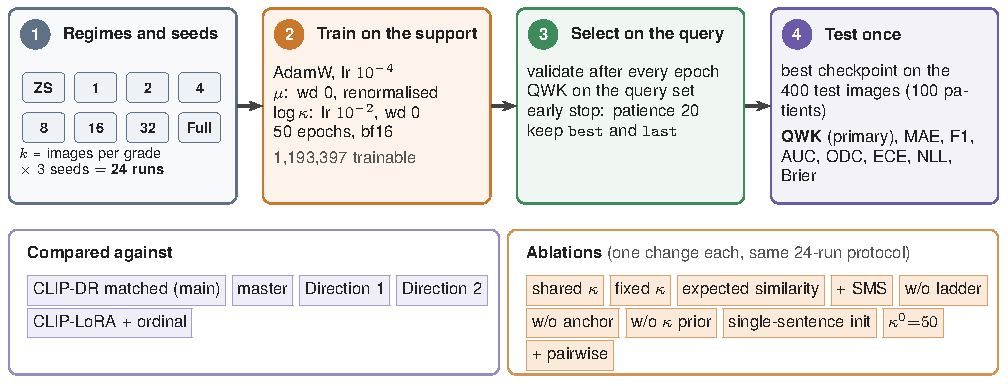
\includegraphics[width=\linewidth]{protocol_d3}
\caption{\lr{protocol} آزمایش‌های جهت ۳.}
\label{fig:proto-d3}
\end{figure}

\begin{figure}[H]
\begin{diagram}
  \node[train=4.4cm] (a) {Phase 1: Dir.~3 · 24 runs};
  \node[box=4.4cm,below=of a] (b) {Compare main models\\ QWK · ODC · ECE · NLL};
  \node[decision,below=of b] (c) {Dir.~3 is best?};
  \node[train=5cm,below=of c] (d) {Phase 2: compare with CLIP-DR \& others + 11 ablations};
  \node[lossn=5cm,below=of d] (e) {Calibration tables and $\kappa$ trajectory per grade};
  \draw[arr] (a)--(b); \draw[arr] (b)--(c); \draw[arr] (c)--node[elabel,right]{yes}(d); \draw[arr] (d)--(e);
\end{diagram}
\caption{گردش کار آزمایش‌های جهت ۳.}
\label{fig:d3-flow}
\end{figure}

\section*{\lr{metric} موفقیت و جمع‌بندی}
\addcontentsline{toc}{section}{\lr{metric} موفقیت و جمع‌بندی}

\begin{keybox}[\lr{metric} موفقیت در هر چهار بخش]
مدلی برتر شمرده می‌شود که در میانگین سه \lr{seed}، \lr{QWK} بالاتری در \lr{regime}های \lr{few-shot} داشته باشد و هم‌زمان در \lr{confusion matrix}‌اش خطاها با دور شدن از قطر کاهش یابند (\lr{ODC} نزدیک به ۱ و \lr{error mass} نزولی بر حسب فاصله). برای جهت ۳، کاهش \lr{ECE} و \lr{NLL} بدون افت \lr{QWK} شرط لازم ادعای \lr{calibration} است.
\end{keybox}

\begin{table}[H]
\caption{مقایسهٔ چهار مدل از نظر اجزا}
\label{tab:summary}
\centering\small
\begin{tabularx}{\textwidth}{@{}p{3.6cm} C C C C@{}}
\toprule
\textbf{جزء} & \textbf{مدل پایه} & \textbf{جهت ۱} & \textbf{جهت ۲} & \textbf{جهت ۳}\\
\midrule
\lr{LoRA} تصویر ($r=16$) & دارد & دارد & دارد & دارد\\
نمایش درجه & \lr{prompt} رتبه‌ای & بردار آزاد & میانگین توصیف‌ها & توزیع \lr{vMF}\\
\lr{text encoder} در آموزش & \lr{frozen}، هر گام & فقط مقداردهی & \lr{LoRA}، هر گام & فقط مقداردهی\\
\lr{CE} + \lr{loss} رتبه & دارد & دارد & دارد & دارد (روی \lr{logit} \lr{vMF})\\
\lr{SMS} & دارد & دارد & دارد & ندارد\\
\lr{ladder} / \lr{anchor} & ندارد & دارد / دارد & دارد / دارد & دارد / دارد\\
\lr{smooth path} & ندارد & دارد & ندارد & ندارد\\
\lr{constraint} ویژه & \lr{interpolation} توکن & مسیر & \lr{description ordering} & \lr{prior} $\kappa$\\
\lr{parameter} \lr{trainable} & \LRE{۱٬۱۹۸٬۰۰۰} & \LRE{۱٬۱۹۳٬۳۹۲} & \LRE{۱٬۲۶۲٬۰۰۰} & \LRE{۱٬۱۹۳٬۳۹۷}\\
\bottomrule
\end{tabularx}
\end{table}

\section*{واژه‌نامه}
\addcontentsline{toc}{section}{واژه‌نامه}
\begin{table}[H]
\caption{معادل‌های به‌کاررفته در سند}
\label{tab:glossary}
\centering\small
\begin{tabular}{@{}ll@{}}
\toprule
\textbf{اصطلاح فارسی} & \textbf{معادل انگلیسی}\\
\midrule
رژیم کم‌نمونه & \lr{few-shot regime}\\
مجموعهٔ پشتیبان / پرس‌وجو & \lr{support / query set}\\
نمونهٔ اولیه & \lr{prototype}\\
توکن بافت / توکن رتبه & \lr{context token / rank token}\\
تطبیق کم‌رتبه & \lr{low-rank adaptation (LoRA)}\\
زیان آگاه از رتبه & \lr{ranking-aware loss}\\
هموارسازی ماتریس شباهت & \lr{similarity matrix smoothing (SMS)}\\
زیان دوتایی وزن‌دار با فاصله & \lr{distance-weighted pairwise loss}\\
کاپای وزنی درجه‌دوم & \lr{quadratic weighted kappa (QWK)}\\
سازگاری افت ترتیبی & \lr{ordinal decay consistency (ODC)}\\
خطای کالیبراسیون مورد انتظار & \lr{expected calibration error (ECE)}\\
لگاریتم درست‌نمایی منفی & \lr{negative log-likelihood (NLL)}\\
توزیع فون‌میزس-فیشر / تمرکز & \lr{von Mises--Fisher distribution / concentration}\\
بسط مجانبی یکنواخت & \lr{uniform asymptotic (Debye) expansion}\\
آزمایش حذفی & \lr{ablation study}\\
\bottomrule
\end{tabular}
\end{table}

\clearpage
\addcontentsline{toc}{section}{منابع}
\begin{latin}
\renewcommand{\refname}{References}
\begin{thebibliography}{99}
\bibitem{clip} A. Radford et al. Learning transferable visual models from natural language supervision. In \emph{ICML}, 2021.
\bibitem{ordinalclip} W. Li et al. OrdinalCLIP: Learning rank prompts for language-guided ordinal regression. In \emph{NeurIPS}, 2022.
\bibitem{clipdr} Q. Yu et al. CLIP-DR: Textual knowledge-guided diabetic retinopathy grading with ranking-aware prompting. In \emph{MICCAI}, 2024.
\bibitem{l2rclip} R. Wang et al. Learning-to-rank meets language: Boosting language-driven ordering alignment for ordinal classification. In \emph{NeurIPS}, 2023.
\bibitem{clap} J. Silva-Rodr\'iguez, S. Hajimiri, I. Ben Ayed, J. Dolz. A closer look at the few-shot adaptation of large vision-language models. In \emph{CVPR}, 2024.
\bibitem{cliplora} M. Zanella, I. Ben Ayed. Low-rank few-shot adaptation of vision-language models. In \emph{CVPR Workshops}, 2024.
\bibitem{lora} E. J. Hu et al. LoRA: Low-rank adaptation of large language models. In \emph{ICLR}, 2022.
\bibitem{fds} Y. Yang et al. Delving into deep imbalanced regression. In \emph{ICML}, 2021.
\bibitem{cupl} S. Pratt et al. What does a platypus look like? Generating customized prompts for zero-shot image classification. In \emph{ICCV}, 2023.
\bibitem{poe} W. Li et al. Learning probabilistic ordinal embeddings for uncertainty-aware regression. In \emph{CVPR}, 2021.
\bibitem{icdr} C. P. Wilkinson et al. Proposed international clinical diabetic retinopathy and diabetic macular edema disease severity scales. \emph{Ophthalmology}, 110(9), 2003.
\bibitem{dlmf} NIST Digital Library of Mathematical Functions, \S10.41: Asymptotic expansions for large order.
\bibitem{deepdrid} R. Liu et al. DeepDRiD: Diabetic retinopathy---grading and image quality estimation challenge. \emph{Patterns}, 3(6), 2022.
\end{thebibliography}
\end{latin}


\end{document}
